\documentclass{article}
\usepackage{floatrow}
\usepackage{float}
\usepackage{multirow}
\usepackage{ragged2e}
\usepackage{indentfirst}
\usepackage{amsmath}
\usepackage{units}
\usepackage{booktabs}
\usepackage{hyperref}
\usepackage{float}
\usepackage{subcaption}
\usepackage{fancyhdr}
\usepackage[utf8]{inputenc}
\usepackage[a4paper,left=2cm,right=2cm,top=2cm,bottom=2cm]{geometry}
\usepackage[utf8]{inputenc}
\usepackage{gensymb}
\usepackage{graphicx}
\usepackage{caption}
\usepackage{wrapfig}
\usepackage[T1]{fontenc}
\usepackage{commath}
\usepackage{empheq}
\usepackage{xcolor}
\usepackage[nottoc]{tocbibind}
\usepackage{url}
\usepackage[portuguese]{babel}
\usepackage{xurl}
\usepackage{multicol}
\numberwithin{equation}{section}
\usepackage{systeme,mathtools}
\usepackage{longtable}
\usepackage{listings}
\usepackage{color} %red, green, blue, yellow, cyan, magenta, black, white
\definecolor{mygreen}{RGB}{28,172,0} % color values Red, Green, Blue
\definecolor{mylilas}{RGB}{170,55,241}
\usepackage{ulem}
\usepackage{setspace}
\onehalfspacing
\usepackage{biblatex}
\usepackage{placeins}
\usepackage{subcaption}
\usepackage{adjustbox}
\usepackage{makecell}
\addbibresource{bib.bib}

\date{March 2021}
\begin{document}



\begin{titlepage}

   \begin{center}
        
\includegraphics[scale=0.3]{Imagens/IST.png} 
        
        \vspace*{0.8cm}
        {\LARGE Licenciatura Bolonha em Engenharia Aeroespacial}
        
        \vspace{1.8cm} 
        \textbf{\LARGE Projecto Integrador de 1º Ciclo em Engenharia Aeroespacial}
        
        \vspace{1.8 cm}
        \noindent\rule{13cm}{0.4pt}
        
        \vspace{0.5cm}
        \textbf{\Huge Urban Air Mobility}

        \vspace{0.3cm}
       {\LARGE Ambulância Aérea}
       
        \noindent\rule{13cm}{0.4pt}
        
        \vspace{3cm}
        
        \large\textbf{GRUPO IV}
       \vspace{0.5cm}

       \large {\textbf{Autores:} 
       \par Joana Filipa Cacilhas de Matos, 95799
       \par João Diogo Queirós Delille, 95800
       \par Pedro Rodrigues Correia da Silva, 95839
       \par Ricardo José Cordeiro Abreu, 95842
       \par Rúben Miguel Duarte Novais, 95843
       \par Tomás Soares e Ribeiro, 95854
       \par Vasco Flores Emídio, 95856
       \par José Miguel Luzia Murteira, 96547}

            
   \end{center}
\end{titlepage}

\clearpage

\fancypagestyle{toc_style}{
\fancyhf{}
%\rhead{\includegraphics[width=15mm]{Imagens/logo_ist.png}}
%\fancyhead[R]{\Large \textbf{Instituto Superior Técnico}  \\ \large \textbf{Projeto Integrador}}

\lfoot{Lisbon DIA MÊS, 2022}
}

\input{Índice}
\pagebreak
\setcounter{page}{1}

\section{Market Study}
Os veículos de emergência providos com equipamento operado por profissionais com formação médica podem ser classificados em:
\begin{itemize}
    \item Transporte terrestre
    \item Asa Rotativa (helicópteros)
    \item Asa Fixa
\end{itemize}

Tanto os veículos de transporte terrestre como as aeronaves de asa rotativa são geralmente utilizados para transportes de curta distância, por exemplo, desde o local onde se encontra o paciente até ao hospital ou entre unidades hospitalares. Já as aeronaves de asa fixa são tipicamente utilizadas para transportes de longa distância, que normalmente requerem deslocamento entre países ou sobre os oceanos.

\textbf{Equipment:}
\begin{itemize}
    \item Bucket-type support with vacuum mattress and patient warming system
    \item Emergency rucksack with special equipment for child and baby care
    \item Portable intensive-care transport respirator \item Oxygen; infection-protection sets
    \item Artificial respiration bag with demand valve, as well as vacuum pumps
    \item Multi-function monitoring
    \item Bi-phase defibrillator, as well as external cardiac pacemakers
\end{itemize}
\par Esta seria uma lista exemplifcativa e, naturalmente, teriam de ser utilizados numerosos equipamentos adicionais de acordo com as condições médicas dos pacientes de modo a assegurar o seu bem-estar.

\textbf{Costs:}

\pagebreak
\section{Concept Generation (Design)}
\subsection{Objective}
Design duma aeronave para funcionar como ambulância aérea. Pretende-se que seja melhor que as ambulâncias aérea atuais de asa rotativa em termos de ruído dentro de espaços urbanos, consumo de combustível, e tempo de resposta a uma emergência.\par
O design híbrido escolhido pretende diminuir o ruído ao usar baterias em descolagem e voo perto do solo, reduzindo o ruído das turbinas geradoras que são utilizadas apenas para voo cruzeiro. O design tilt-rotor permite aumentar significativamente a eficiência em voo horizontal e permite um aumento moderado da velocidade de cruzeiro quando comparado com helicópteros convencionais. \par
Deverá ter pelo menos o mesmo alcance que o AW 139, bem como levar o mesmo número de passageiros e crew members.\par
Deverá operar em zonas suburbanas e urbanas.\par
Dada a infraestrutura atual, deverá ocupar no máximo um circulo de 14 metros (limite imposto por heliportos existentes)\par
Deverá carregar pelo menos 150kg de material médico (dados de \textit{market study} - valor baseado no \textit{weight limit} para equipamento médico para aeronaves como Citations, Pilatus PC12 e Eurocopter AS350, bem como no documento \textit{Specification of Equipments for ERS Ambulance}, NHM) %INSERIR REFERÊNCIA BIBLIOGRAFIA 
%(dados da market study team - Joana help)

Deverá ter um tempo de preparação para descolagem menor do que helicópteros atuais, o que se pretende alcançar ao usar motores elétricos em vez de um sistema puramente mecânico.\par

\subsection{Mission}
A overall missão que este design procura realizar é a de: 
\begin{itemize}
    \item Ir do hospital para o local da emergência
    \item Assistência médica
    \item Levar o paciente para o hospital onde receberá assistência (não necessariamente o de partida)
    \item Regressar à base
\end{itemize}
Esta é partida em secções menores:
\begin{itemize}
    \item 
    \item
    \item
    \item
    \item
\end{itemize}
\subsection{Cenas de referância}
 Aeronaves de referencia
    \begin{itemize}
        \item AW 139
         \begin{itemize}
            \item Dimensionamente geral duma ambulância aérea
            \item Generator reference - quantidade (2 geradores) e potencia (2MW cada)
            \item Shape da fuselagem
            \item Cargo
            \item Reference for how good the replacement has to be - we are trying to match or beat this helicopter in terms of noise fuel and everything
            \item Dry mass/structural weight
        \end{itemize}
        
        \item XV 15
            \begin{itemize}
            \item Dimensionamento de motores e combustivel estimado para um veiculo VTOL de 6T de MTOW
            \item Dimensionamento de fuselagem e cargo para veiculos VTOL
            \item Inspiração -> Honestly, deviamos só usar o XV-15 e pronto
            \item 
        \end{itemize}
        
        \item V-22
        \begin{itemize}
            \item Fonte de vários dados sobre caracteristicas de VTOL e perfis de voo para este tipo de veiculo
        \end{itemize}\textbf{}
        
        \item V-280
        \begin{itemize}
            \item Estudo de mecanismos alternativos para tiltrotors
        \end{itemize}
        
        \item X-19
        \begin{itemize}
            \item Estudo sobre a viabilidade de rotores distribuidos em configuração de quadcopter
            \item inspiração
        \end{itemize}
        
        \item Lillium Jet
        \begin{itemize}
            \item Inspiração para ducteded distribution propultion
            \item motores eletrico + propeller em cima da asa. Um motor por propeller
            \item esteira convergente (no ducto)
        \end{itemize}
        \item Sugar Volt
        \begin{itemize}
            \item Descritização da massa - uso duma tabela com as massas de vários componentes para ter ideia dos rácios entre a massa total e a asa e a fuselagem.
        \end{itemize}
    \end{itemize}
Peças
\begin{itemize}
    \item Motores electricos (referência de mercado)
    \begin{itemize}
        \item 17 kg
        \item 80kW
    \end{itemize}
\end{itemize}
\section{Designs}
As primeiras proposta teviram as seguintes ideias em mente:
\begin{itemize}
    \item Ocupar um circulo de 14m
    \item Utilizar conventional wing ou tadem wing
    \item Asa alta
    \item 8 motores eletricos (4 em cada asa no conventional, 2 em cada no tandem)
    \item 2 geradores eletricos de 1 MW cada
    \item Porta lateral
    \item T tail configuration on the conventional wing design
    \item Fuselage shape baseada no AW 139
    \item Tilt rotor
\end{itemize}

Baseado nisto, foram propostas mais duas configurações. Estão são quase idênticas às em cima descritas, mas utilizam multiplas ducted fans para boundary layer ingestion, baseado no lillium jet. Também estas fans têm um mecanismo de tilt para permitir VTOL bem como horizontal cruise flight com essas na horizontal.

\section{Semana 1 - Market Study and Concept Generation}
\subsection{Market Study}
\textbf{\Large{Metam aqui o market study}}
\subsection{Concept Generation}
\subsubsection{Introdução}
A geração de conceitos (\textit{Concept Generation}) inicial é um processo no qual se utilizaram aeronaves já existentes, bem como conhecimentos prévios nos domínios de engenharia para gerar conceitos gerais preliminares, ou seja, com poucas especificações, para a aeronave que deverá ser \textit{designed} no final do trabalho. Este processo culminou na criação de dois desenhos feitos sem escala em papel à mão.\par
\subsubsection{Aeronaves Históricas}
A recolha de Aeronaves baseou-se em dois fatores: estudo de mercado e tipos de descolagem.\par
\paragraph{Descolagens}
Inicialmente, considerou-se que Short Take Off and Landing (STOL) poderia ser uma opção. No entanto, sendo que o estudo de mercado se focou num meio totalmente urbano, foi claro que este método não poderia ser utilizado devido à necessidade de aterrar no meio de espaços urbanos. Para tal, Vertical Take Off and Landing (VTOL) foi escolhido. Este, além de assegurar que é possível aterrar em estradas e espaços pequenos, também permite a utilização de heliportos já existentes em hospitais e outros edifícios.\par
Este último facto veio a enfatizar que se poderia utilizar a infraestrutura já existente para helicópteros utilizados como ambulâncias aéreas. Tal será relevante noutras parte do relatório, nomeadamente, mission design na Semana 2 e nas restrições nas dimensões máximas ao longos das iterações de \textit{designs}. A utlização desta infraestrutura veio a impor um tamanho máximo de 14 metros em qualquer direção horizontal daqui em diante, apesar de tal não ser considerado nesta semana.\par
\paragraph{AW139}
%Dada a necessidade de VTOL e a existência de ambulâncias aéreas com esta possibilidade, foram considerados os helicópteros utilizados em serviços de urgência.

Tendo em conta o objetivo de realizar descolagens e aterragens verticais, procuramos primeiro encontrar dados de helicópteros já utilizados como ambulâncias aéreas. A pesquisa culminou na escolha do Agusta-Westland AW139 como referência para os nossos estudos, utilizado em \textbf{\large{Inserir onde é utilizado + citação; inserir as outras alternativas e o pq de não as escolhermos}}.\par
\FloatBarrier
\begin{figure}[h]
    \centering
    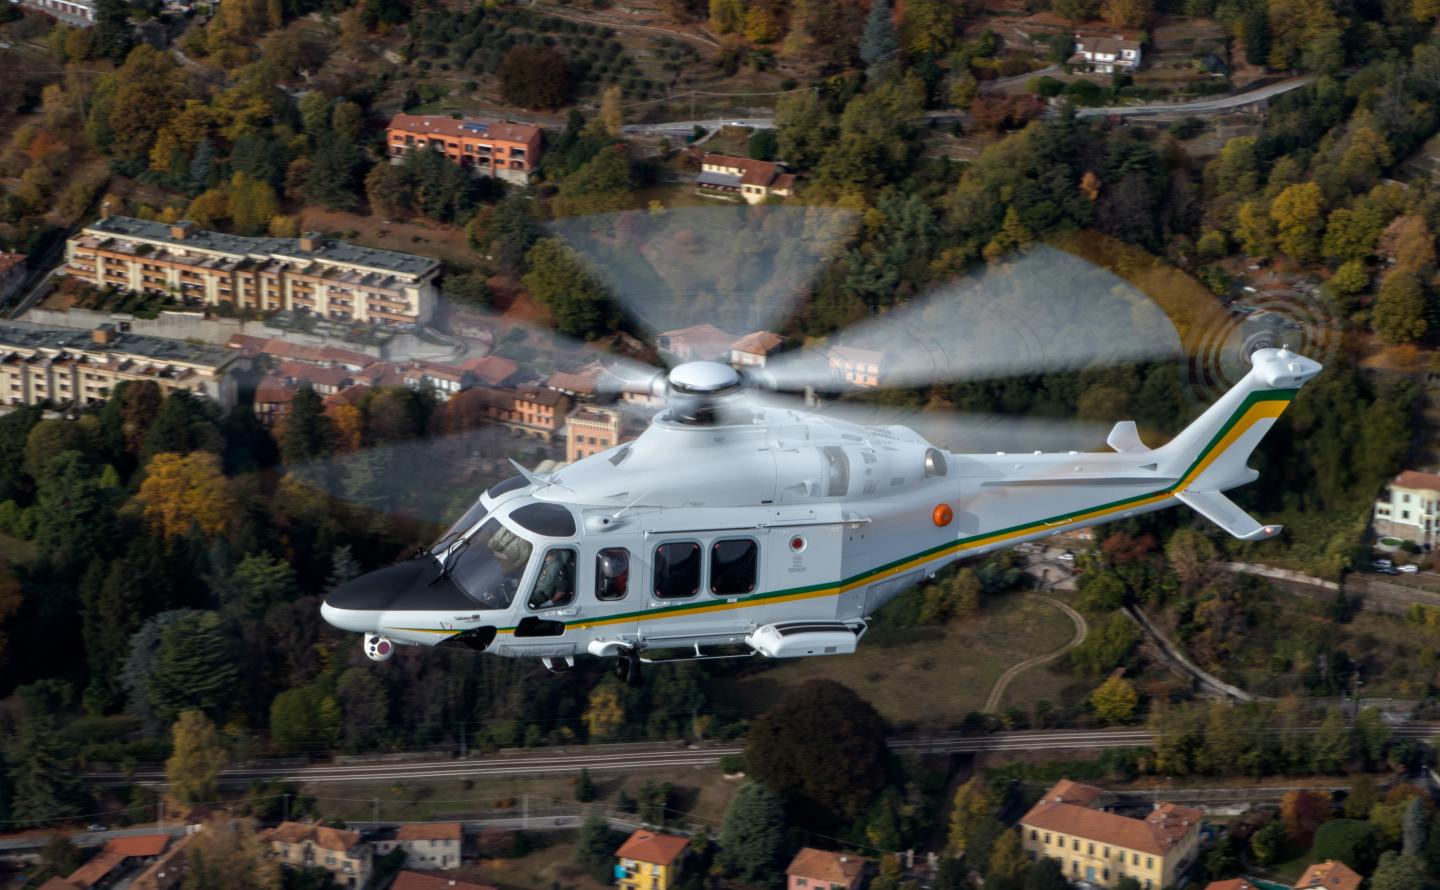
\includegraphics[width=0.5\textwidth]{Imagens/aw139.jpg}
    \caption{AgustaWestland AW139 Source:\cite{noauthor_undated-ue}}
    \label{fig:my_label}
\end{figure}
\FloatBarrier
Este helicópero apresenta as seguintes caracteristicas (Source:\cite{noauthor_undated-ue}):
\begin{table}[h]
\begin{tabular}{|l|l|}
\hline
Max Gross Weight                                                                                             & 6,400 kg 14,110 lb                                   \\ \hline
Increased Gross Weight                                                                                       & 6,800/7,000 kg 14,991/15,432 lb                      \\ \hline
Powerplant                                                                                                   & 2 x Pratt \& Whitney PT6C-67C Turboshafts with FADEC \\ \hline
Overall length (Rotors Turning)                                                                              & 16.66 m 54 ft 08 in                                  \\ \hline
Overall height (Rotors Turning)                                                                              & 4.98 m 16 ft 04 in                                   \\ \hline
Rotor diameter                                                                                               & 13.8 m 45 ft 03 in                                   \\ \hline
Capacity                                                                                                     & Crew 1-2 Passengers up to 15                         \\ \hline
Max Cruise Speed (ISA, MGW, SL, MCP)                                                                         & 305 km/h 165 kt                                      \\ \hline
HIGE (ISA, MGW, TOP)                                                                                         & 4,672 m 15,327 ft                                    \\ \hline
HOGE (ISA, MGW, TOP)                                                                                         & 2,476 m 8,123 ft                                     \\ \hline
\begin{tabular}[c]{@{}l@{}}Max Range (ISA, MGW, SL)\\ with auxiliary fuel tank - No reserve\end{tabular}     & 1,032 km 557 nm                                      \\ \hline
\begin{tabular}[c]{@{}l@{}}Max Endurance (ISA, MGW, SL)\\ with auxiliary fuel tank - No reserve\end{tabular} & 5 h 05 min                                           \\ \hline
\end{tabular}
\end{table}
\FloatBarrier
A massa máxima, bem como o \textit{max cruise speed} foram consideradas métricas importantes para comparar com o nosso design. 

%>>>>>
O nosso objeto era conseguir uma velocidade de cruzeiro superior com um veículo de menor massa, de forma a obter uma alternativa viável às soluções existentes.\par
% A velocidade de cruise deveria ser ultrapassada a fim de ser mais viável a nossa configuração e a massa deveria ser menor, conseguindo um design mais leve.\par
%<<<<<

A utilização duma powerplant igual à do AW139, constítuida por dois Turboshafts de 1 MW cada colocadas no topo da fuselagem \textbf{(citação??)} foi considerada para o nosso design como uma possibilidade (que acabou por ficar em todos as futuras iterações). 

%>>>>>
Apesar de neste ponto não ser considerada uma forma de propulsão em particular, foi considerado que caso se optasse por qualquer tipo de propulsão híbrida esta powerplant seria viável pois é uma configuração comum em helicópteros e a potência é semelhante à do XV-15, um tiltrotor de MTOW semelhante ao AW139 que também foi usado como referência na nossa pesquisa.\par
%Apesar de ainda, neste ponto, não se ter considerado uma arquitetura de propulsão, foi considerado que caso se optasse por uma turboeletrica ou com multiplos rotores e uma single power sorce, se poderia utilizar estas turbinas. Além de tal, foi considerada a sua posição, concluindo-se que se poderia utilizar a mesma localização, no topo da fuselagem, embedded.\par
%<<<<<

Além destes pormenores, a forma geral da fuselagem será parcialmente baseada no design do AW139.\par

\paragraph{Tilt Rotors and Tilt Wings}

%>>>>> refazer wording
No processo de geração de conceitos, procurou-se encontrar designs que seriam melhores que o helicóptero. Para tal, teve-se a ideia de que se poderia ter um cruise mais rápido e eficiente se se utiliza-se uma configuração parecida a um avião de asa fixa {\large{\textbf{Inserir citação or something sobre aviões serem melhores em cruise}}}. No entanto, sendo um avião e não um helicóptero, é necessário definir uma forma de ele realizar VTOL.\par
A pesquisa de configurações já existentes com estas qualidades resultou em ter em conta 3 aviões: XV-15, Bell Boeing V-22 Osprey, Bell V-280 Valor e LTV XC-142.\par
%<<<<< refazer wording 

O XV-15 foi um avião exprimental da NASA Tilt Rotor capaz tanto de descolagem vertical como voo horizontal, em modo de \textit{hover} ou \textit{cruise}.\cite{Maisel2001-fz} Estes modos estão apresentados na figura abaixo, aplicando-se em geral a tilt rotors.
\FloatBarrier
\begin{figure}[h]
    \centering
    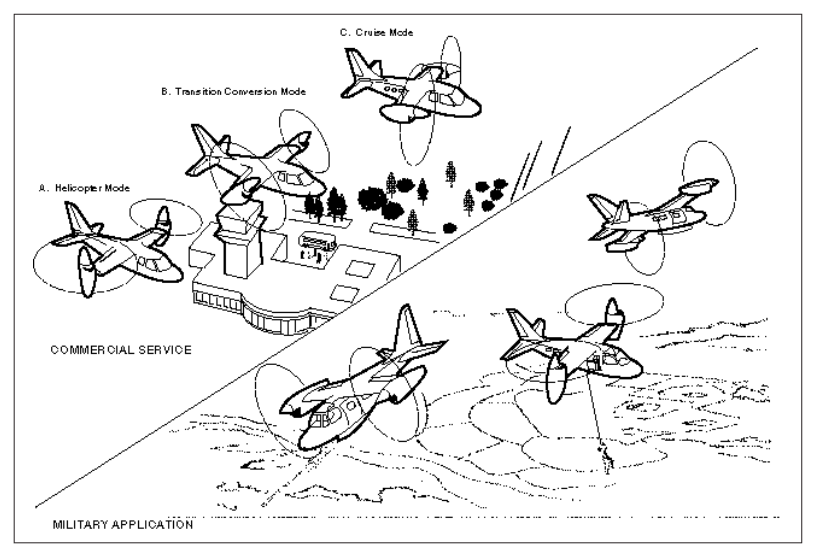
\includegraphics[width=0.7\textwidth]{Imagens/tiltrotor.PNG}
    \caption{"Illustration from 1974 Tilt Rotor Research Aircraft Project PlanSource":\cite{Maisel2001-fz}}
    \label{fig:my_label}
\end{figure}
\FloatBarrier
Dado estes modos de operação, bem como a capacidade de VTOL, este modelo impulsionou a solução de utilizar uma configuração tilt rotor no design. É apresentado, em baixo, o XV-15 a voar, de forma a enfatizar o facto de ser uma tecnologia testada que funciona. 

%>>>>>
Além de ter dois modos de voo, os rotores podem ser rodados para qualquer ângulo intermédio de modo a garantir eficiência máxima para todas as velocidades de voo.\cite{Maisel2001-fz}. 
%Além de tal, é importante referir que ele consegue voar com o "titl" intermédio, podendo escolher voar de forma mais eficiente a baixas velocidades.\cite{Maisel2001-fz}. 
%<<<<<

Tal funcionalidade também é tida em conta na escolha de usar um tilt rotor.\par 


\FloatBarrier
\begin{figure}[h]
    \centering
    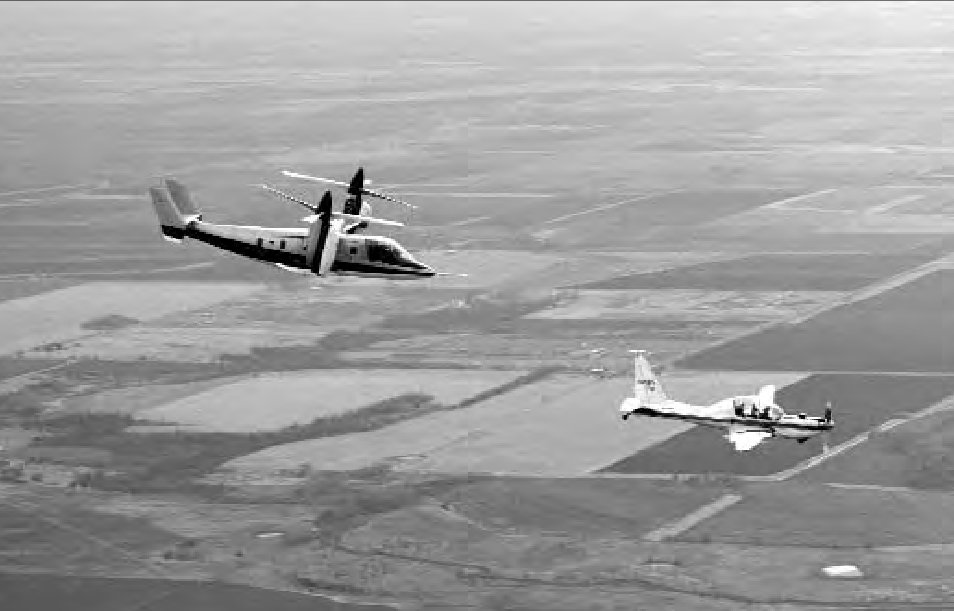
\includegraphics[width=0.5\textwidth]{Imagens/xv-15 cruise.PNG}
    \caption{"The XV-15 flying in close
formation with the YO-3A
for acoustics data.
(Ames Photograph
AC95-0438-15.1) Source:\cite{Maisel2001-fz}"}
    \label{fig:my_label}
\end{figure}
\FloatBarrier
O Bell Boeing V-22 Osprey é uma outra aeronave \textit{tilt rotor} considerada neste relatório. Neste caso, não é exprimental, sendo largamente utilizada, nomeadamente no contexto militar. Tal, mais uma vez, vem a viabilizar o tilt rotor como escolha possível.\par
{\large{\textbf{SOMEHOW É SUPOSTO MENCIONAR PERFIS DE VOO? Delille, completa, que tinhas dito isso}||| ze do que é que estas a falar what eu disse o que de que perfis de voo? tas a falar do facto de poder voar com angulos diferentes de tilt? like, ja mencionamos isso no xv15, dizemos so "tal como o xv15 o v22 tb faz angulos intermedios?? quais perfis de voo"}}\par
O Bell V-280 Valor, também uma aeronave tilt-rotor da Bell, criada como sucessor do V-22 com o objetivo de corrigir problemas no seu design original, é considerado como de importância devido ao uso de um "Non-Rotation Engine".\cite{noauthor_undated-gb}. Em baixo, de forma a ser mais claro, é apresentado a imagem de tanto a aeronave como desta informação, presente no site oficial da Bell.\par
\FloatBarrier
\begin{figure}[h]
    \centering
    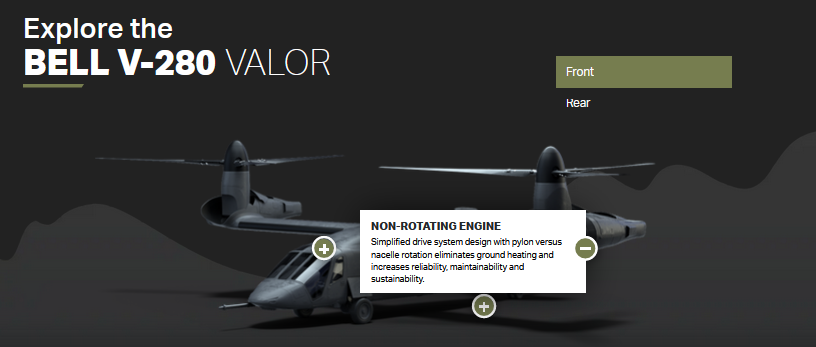
\includegraphics{Imagens/v_280.PNG}
    \caption{V-280 Source:\cite{noauthor_undated-gb}}
    \label{v-280}
\end{figure}
\FloatBarrier
Esta forma de girar os rotores de forma a se poder realizar VTOL, permite o uso de motores não só no centro das asas, o que não seria possivel se se rodasse a nacela do motor inteira. É de notar, no entanto, a interferência da asa com a esteira do rotor quando este está em posição vertical. Isto pode ser mitigado ao afastar o rotor da asa para permitir que a asa obstrua uma menor área do rotor.\par
O LTV XC-142 foi o único exemplo de uma aeronave de asa fixa VTOL encontrado durante a pesquisa que faz uso de \textit{tilt wings} em vez de \textit{tilt rotors}. {\Large{\textbf{Inserir citações, nomeadamente sobre como tilt wing é uma autentica complicação mecanica e tal}}}.\par
\subsection{Inicial Concept}
Inicialmente, foram realizados dois designs, em baixo apresentados.
\FloatBarrier
\begin{figure}[h]
    \centering
    \begin{subfigure}[b]{0.47\textwidth}
        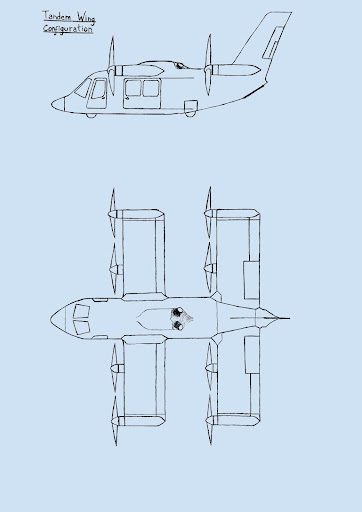
\includegraphics[width=\textwidth]{Imagens/inicialdesign1.jpg}
        \caption{Primeiro Design Sketch 1}
        \label{DesingSketchini1}
    \end{subfigure}
    \hfill
    \begin{subfigure}[b]{0.47\textwidth}
        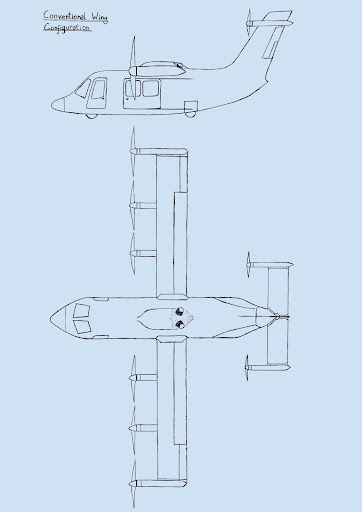
\includegraphics[width=\textwidth]{Imagens/inicialdesign2.jpg}
        \caption{Primeiro Design Sketch 2}
        \label{DesingSketchini2}
    \end{subfigure}
    \caption{Conceitos Iniciais - Semana 1}
\end{figure}
\FloatBarrier
Ambos os esboços apresentam uma fuselagem alongada, com um nariz semelhante ao AW139. No entanto, como não é necessário um rotor de cauda para controlar a guinada, em vez de ter uma cauda estreita e alongada foi escolhida uma cauda mais curta com maior volume interno semelhante a um avião convencional, na qual assenta o estabilizador horizontal. Apresentam, igualmente, uma porta lateral, como no AW139.\par
Notar que os desenhos são puramente qualitativos e não apresentam proporções ou posições exatas das várias partes. Tendo tal em conta, nota-se que as pás dos rotores da asa da figura \ref{DesingSketchini2} encontram-se em frente à porta, o que não deverá acontecer no design final.\par
Ambas as configurações, apesar de não estar explícito nos desenhos, deverão apresentar a configuração tilt rotor presente no Bell V-280.\par
O trem de aterragem é baseado no AW139, sendo triangular.\par
A grande diferença entre as duas configurações é o facto de a primeira ser Tandem Wing, enquanto que a segunda apresenta uma configuração convencional com a cauda em cruz. O estabilizador vertical é colocado acima da asa principal na figura\ref{DesingSketchini2} de forma a diminuir a interferência nesse mesmo por ela causada.\par
%>>>>>
A configuração \textit{tandem wing} é proposta como solução para o problema da restrição de tamanho imposta pelos heliportos, pois receávamos que para obter uma área de asa suficiente para sustentar a aeronave em voo cruzeiro esta teria de ter uma envergadura demasiado longa para caber dentro de um heliporto, ou teria de ter uma corda tão grande que não seria eficiente. Usando uma \textit{tandem wing} a área da asa é efetivamente duplicada mantendo a mesma corda e envergadura, no entanto é difícil de estimar o ganho de eficiênicia relativamente a simplesmente duplicar a corda.\par
Além disto, esta configuração combinada com preciso controlo eletrónico do impulso gerado por cada rotor permite um melhor controlo de atitude em \textit{hover} devido à maior distância entre os rotores e o centro de massa.\par
%A tandem wing é proposta devido à restrição de tamanho do heliporto, dado que não é possivel ter uma asa com alto aspect ratio e obter a mesma área que a conseguida com a tandem wing. Apesar de ser mais ineficiente em geral do que apenas uma asa com maior aspect ratio, dado que esse pode não ser possível, coloca-se a hipótese cuja validade só poderá ser averiguada em estudos posteriores a esta fase.\par
%Além disto, esta configuração também permite uma distribuição mais equilibrada durante o VTOL devido ao quadcopter.\par
%<<<<<
Nesta fase, considerou-se propulsão puramente turboelétrica em que um gerador alimenta os motores diretamente sem intermediários, não sendo menicionadas, por isso, baterias.\par
\section{Semana 2 - Market Opportunities, Costs, Addicional Design Generation and Analytic Hierarchy Process (AHP)}
\subsection{Market Opportunities}
\subsection{Costs}
\subsection{Addicional Design Generation}
\subsubsection{Introdução}
Na semana dois, foi necessário realizar o Analytic Hierarchy Process (AHP). Este consiste num método para avaliar designs comparativamente. Dado que foi decidido que este deveria avaliar quatro designs, consideramos outros dois adicionais para além dos detalhados na secção referente à semana anterior a esta.\par

\subsubsection{Lillium jet, ductos, e aviões elétricos}
Dada a convencionalidade do dois primeiros designs esboçados, de forma a procurar criar conceitos variados para o AHP, foi decidido investigar aeronaves menos convencionais, nomeadamente no ramo de mobilidade urbana e regional. Dever-se-á notar que, primeiramente, foi focada a procura de soluções puramente a combustão e baseado em aeronaves exprimentais e já em serviço, de forma a confirmar a viabilidade das nossas escolhas. Alargou-se, assim, neste ponto do trabalho, a procura, em particular, para eVTOL.\par
Vários designs existentes de veiculos eVTOL foram considerados e uma lista dos candidatos que pareceram mais viáveis e mais interessantes para o nosso projeto foi compilada:
\begin{itemize}
    \item Joby S4 - pelo mecanismo de tilt rotor
    \item NASA Greased Lightning - pelo mecanismo de tilt wing
    \item NASA LA-8 - pelo mecanismo de tilt wing e tandem wing
    \item HopFlyt Venturi - pelo design de channel wings e tandem wing
    \item Airbus A³ Vahana - pelo design tandem wing extremamente semelhante ao inicialmente considerado
    \item Bell Nexus 6HX - pelo design de ducted fans
    \item Lillium Jet - pelo design de tandem wing com micropropulsão de ducted jets 
\end{itemize}
Desta pesquisa resultou a escolha do Lillium Jet como referência, dado ser uma das aeronaves mais avançadas no seu desenvolvimento, e com características que melhor se alinhavam com os nossos objetivos, nomeadamente o seu pequeno tamanho juntamente com a redução de ruído e aumento de eficiência e segurança prometidos pelo seu design de jatos elétricos. 
O Lillium Jet apresenta uma configuração fixed wing com canard, puramente elétrica de propulsão distribuída com jatos em ductos embebidos que podem ser rodados para descolagem e aterragem vertical. Uma imagem representativa é apresentada em baixo.\par
\FloatBarrier
\begin{figure}[h]
    \begin{subfigure}[t]{0.47\textwidth}
        \centering
        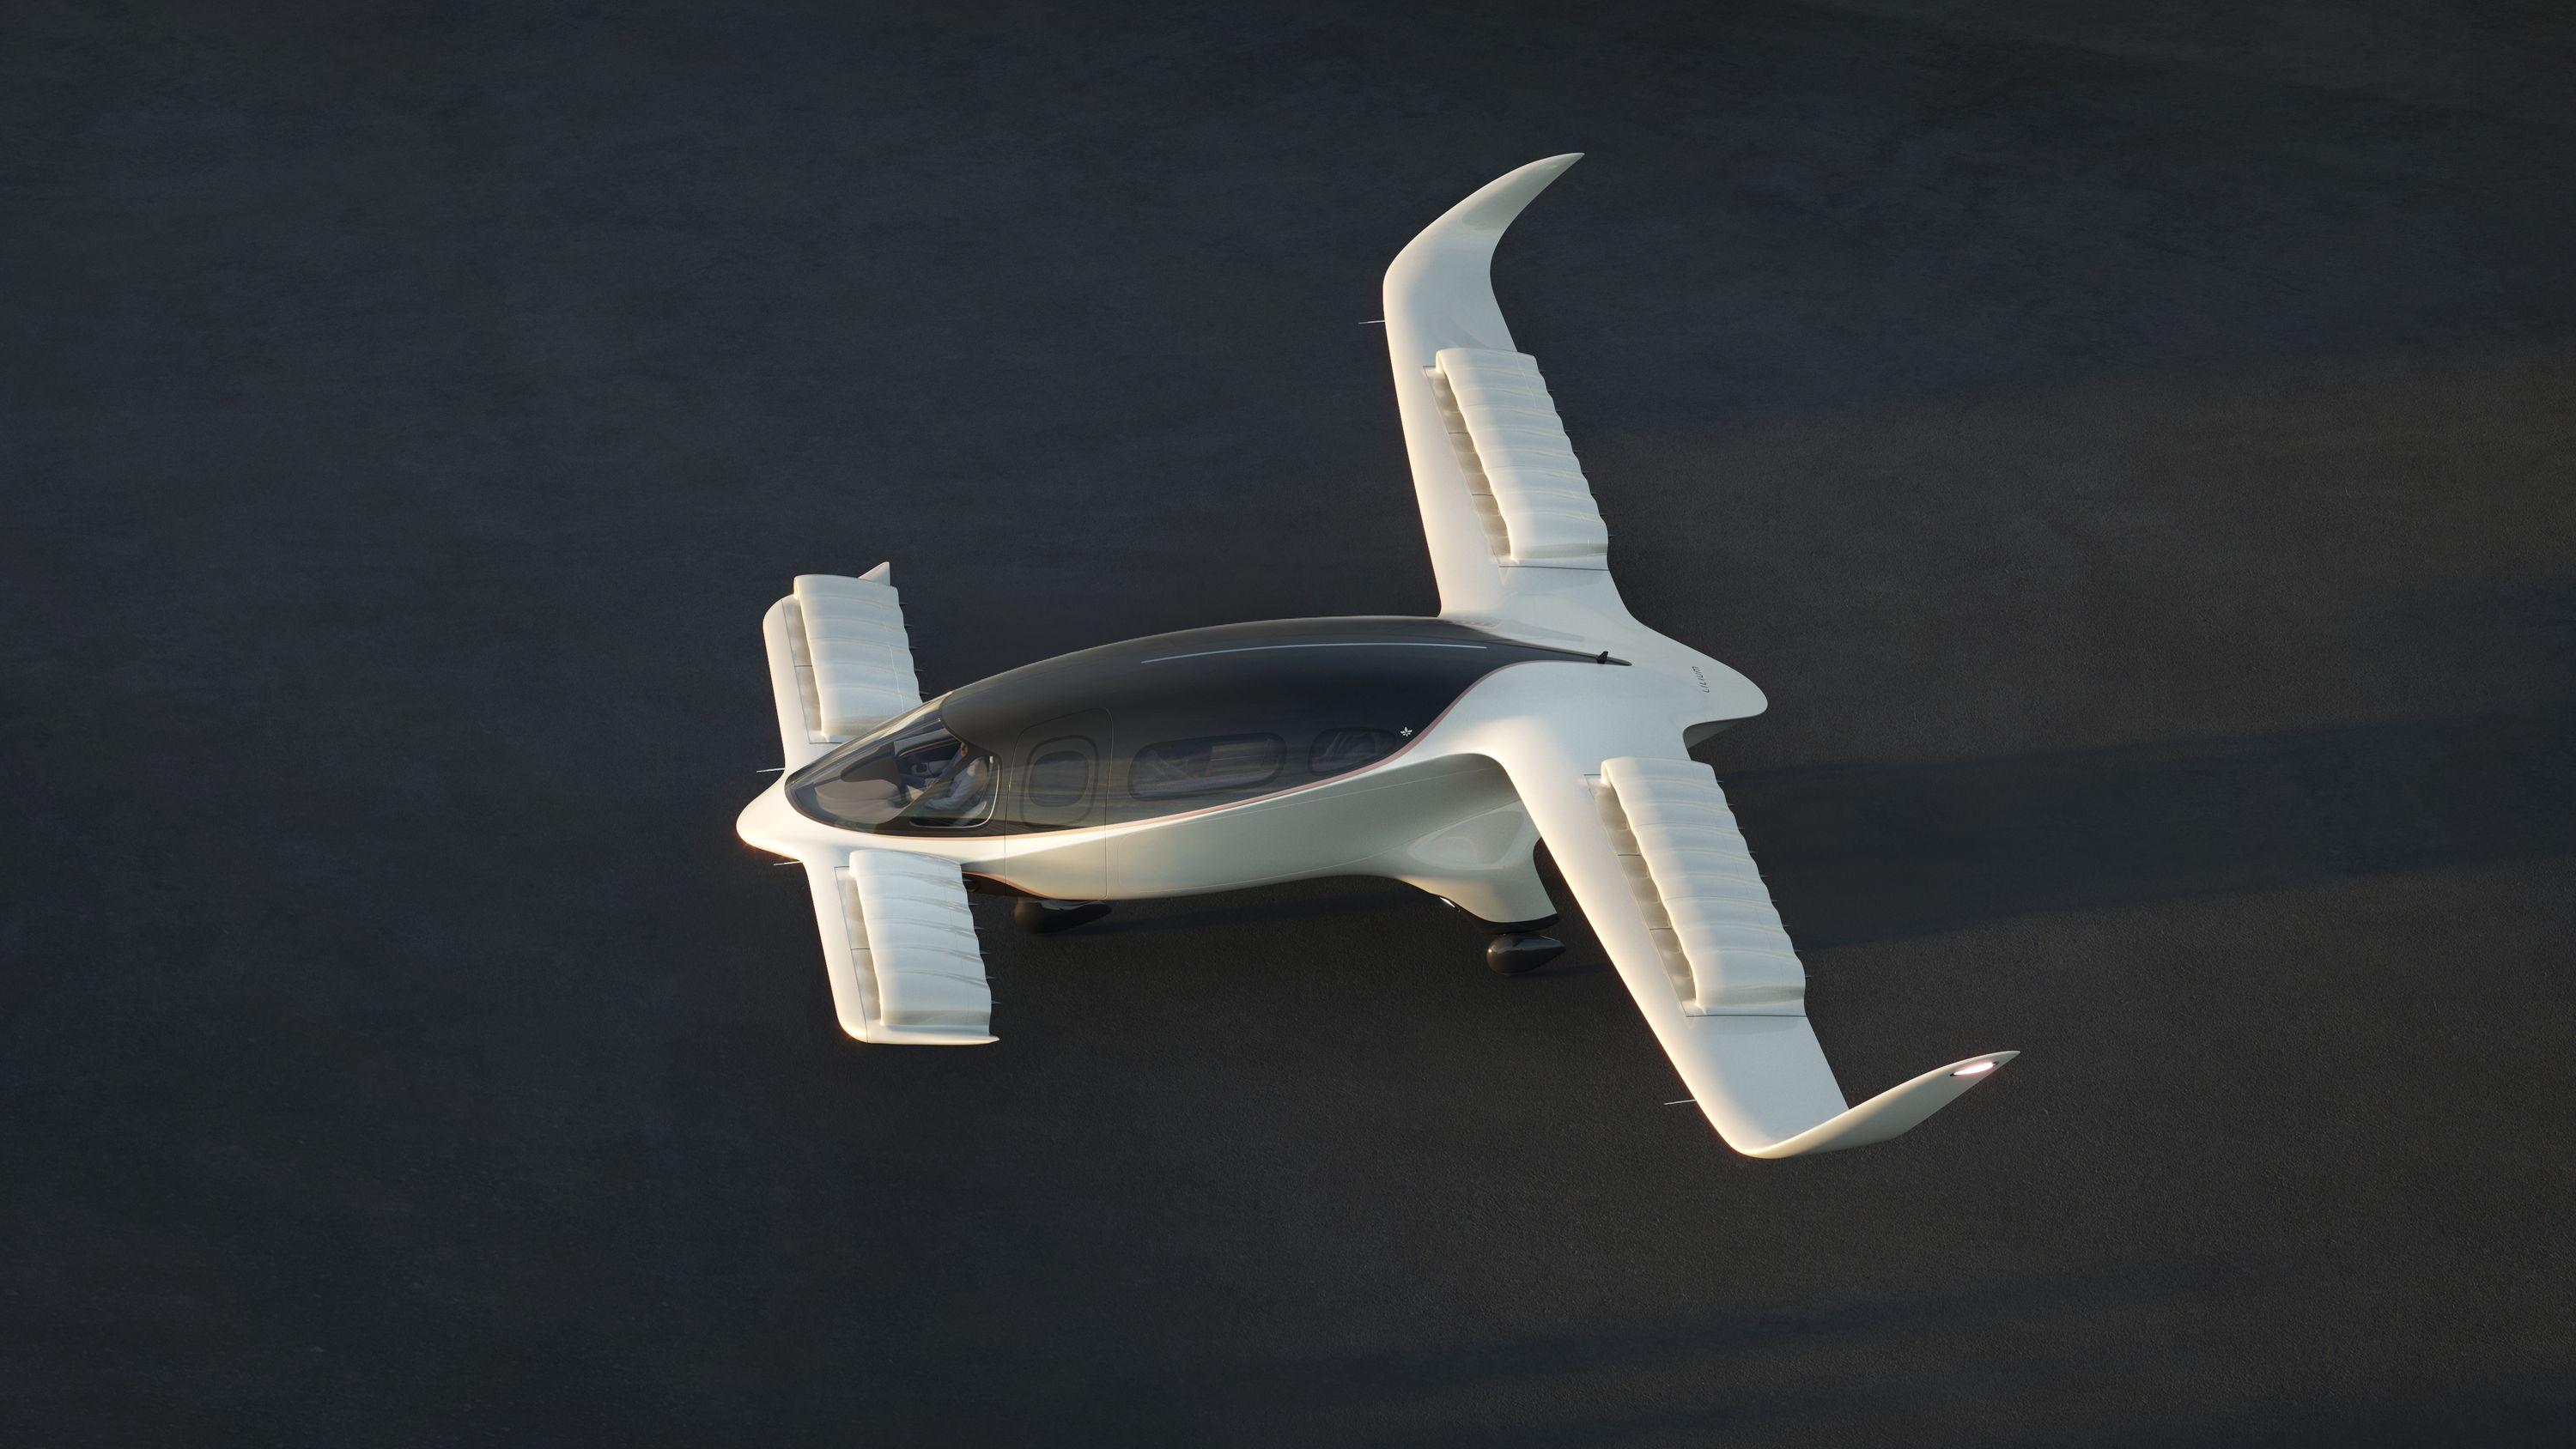
\includegraphics[width=\textwidth]{Imagens/Lilium-Jet-Top-Side_result1.jpg}
        \caption{Lillium Jet Source:\cite{noauthor_2022-ne}}
        \label{LilliumJet}
    \end{subfigure}
    \hfill
    \begin{subfigure}[t]{0.47\textwidth}
        \centering
        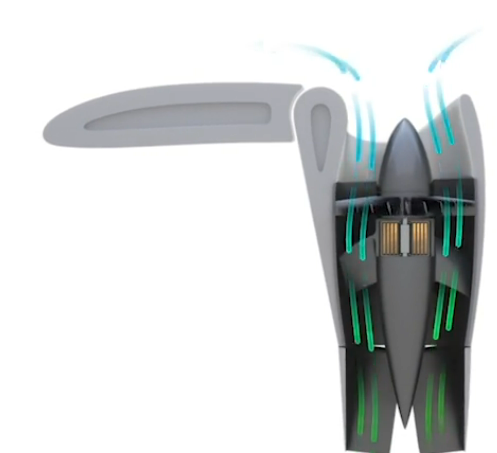
\includegraphics[width=\textwidth]{Imagens/tiltrotorlillium.PNG}
        \caption{Lillium Jet Source:\cite{noauthor_2022-ne}}
        \label{LilliumJettiltrotor}
    \end{subfigure}
    \caption{Lillium Jet e detalhe da propulsão}
\end{figure}
\FloatBarrier
O uso de jatos em ductos sobre a asa deve resultar numa maior eficiência em todo o perfil de voo bem como numa redução de ruído durante a operação. Tal se deve à diminuição das interações entre os rotores e o isolamento acústico inerente a cobrir os rotores, à diminuição dos números de Mach locais (equivalente a permitir que os rotores possam rodar mais rapidamente, melhorando a sua eficiência), ao uso de tubeiras convergentes para obter maior impuslo com um rotor menor, e ao facto de que ao estarem colocados no bordo de fuga acelerarem o o ar sobre a asa, criando lift adicional. Têm no entanto a desvantagem de adicionarem peso e complexidades estruturais à aeronave, além de serem mais difíceis de prever aerodinamicamente ao contrario de configurações convencionais. {\large{\textbf{citaç~eos para isto tudo, s'il vous plait}}}\par
Além da existência de ductos, este desgin também se distingue ao usar 36 pequenos motores elétricos distribuídos ao longo da asa e do canard.
Tendo em conta o apresentado, foi considerado que o fator mais distinto e importante era o sistema de propulsão, pelo que se baseou os novos designs nos primeiros, modificando-os para fazerem uso de tilt jets embebidos na asa, tal como o Lillium Jet. Em baixo encontram-se os novos designs apresentados na segunda semana.
\FloatBarrier
\begin{figure}[h]
    \centering
    \begin{subfigure}[b]{0.47\textwidth}
        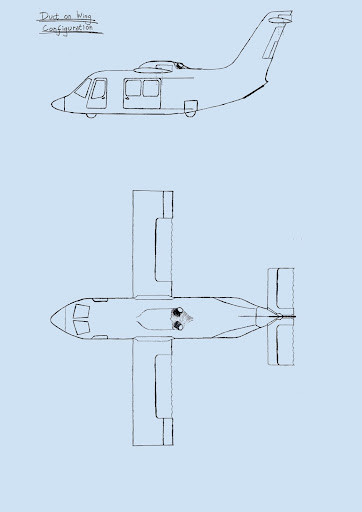
\includegraphics[width=\textwidth]{Imagens/segundodesign1.jpg}
        \caption{Segundo Design Sketch 1}
        \label{SecondDesingSketchini1}
    \end{subfigure}
    \hfill
    \begin{subfigure}[b]{0.47\textwidth}
        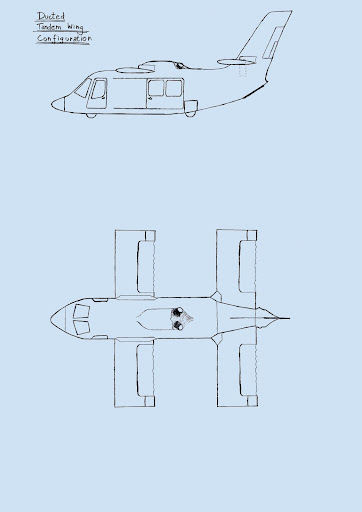
\includegraphics[width=\textwidth]{Imagens/segundodesign2.jpg}
        \caption{Segundo Design Sketch 2}
        \label{SecondDesingSketchini2}
    \end{subfigure}
    \caption{Conceitos com propulsão distribuída  - Semana 2}
\end{figure}
\FloatBarrier
Dever-se-á notar, então, que, no topo das asas, encontram-se motores elétricos de dimensões menores aos apresentados na semana um. Estes, tal como no Lillium Jet, encontram-se no bordo de fuga e deverão ter como exequivel a mudança de orientação através dum mecanismo semelhante àquele presente no Lillium Jet, em particular expressado na figura \ref{LilliumJettiltrotor}.\par
\subsection{Analytic Hierarchy Process (AHP)}
\textbf{HOnestamente, não me apetece escrever isto pq eu nem percebi bem o pq de decidirmos que certos parametros são melhores que os outros, so ya||| pois eu tb nem quero ter de me lembrar que sequer fizemos esta parvoice da AHP de adivinhar o que era bom e mau para depois concluirmos "adivinhamos errado"}
\section{Semana 3 - Mission Profile + MTOW Estimation}
\subsection{Introdução}
Nesta secção, apresenta-se a missão bem definida da nossa aeronave bem como o Maximum Take Off Weight (MTOW).\par
Nesta semana foi introduzido um programa escrito em Matlab fornecido aos alunos. Este possibilita o cálculo do design point bem como a estimação de múltiplos parâmetros baseado em equações de desempenho e valores empíricos. A falta de documentação do programa e de comentários no source code levou a que certas funcionalidades e dados não tinham sido utilizados imediatamente, dado terem sido encontrados posteriormente. Além de tal, limitações do programa bem como a inexistência de equações empíricas para certos designs limitou a escolha de design, dada a impossibilidade de estimar valores para esses casos.\par
\subsection{Mission Profile}
{\large{\textbf{Inserir todas as cenas e citações sobre como chegamos ao mission desgin, pq eu não sei onde fomos buscar os dados}}}\par
A Missão ficou definida como a composição de três partes:
\begin{itemize}
    \item Levar material médico e paramédicos do hospital inicial até ao local da emergência
    \item Levar o paciente, juntamente com os paramédicos e o material médico, para um hospital especializado/especifico.
    \item Regressar ao hospital inicial
\end{itemize}
Apesar de ser possível regressar ao hospital inicial, tal não é assumido, devido ao facto de tal não ser nem sempre nem necessariamente o caso, pelo que, de forma a criar a missão mais geral possível, escolheu-se a supracitada.\par
Cada troço é iniciado por uma secção de taxi, estando a aeronave preparada para descolar, no chão, ligada a aguardar. Este é de larga importância devido à queima de combustível associada. A aeronave foi projetada com o objetivo \textbf{inserir estudo que não me lembro qual era} de ter um dispatch time menor que a de um helicóptero de forma a ser mais eficiente e viável para menores distâncias. Notar que, para menores distâncias, devido ao tempo de dispatch, pode ser mais viável utilizar uma ambulância terrestre, inviabilizando o nosso design nesses casos. Diminuir este tempo, então, alarga a variedade de missões que ela pode realizar.\par

Apresenta-se, em baixo, o esboço da missão.
\FloatBarrier
\begin{figure}[h]
    \centering
    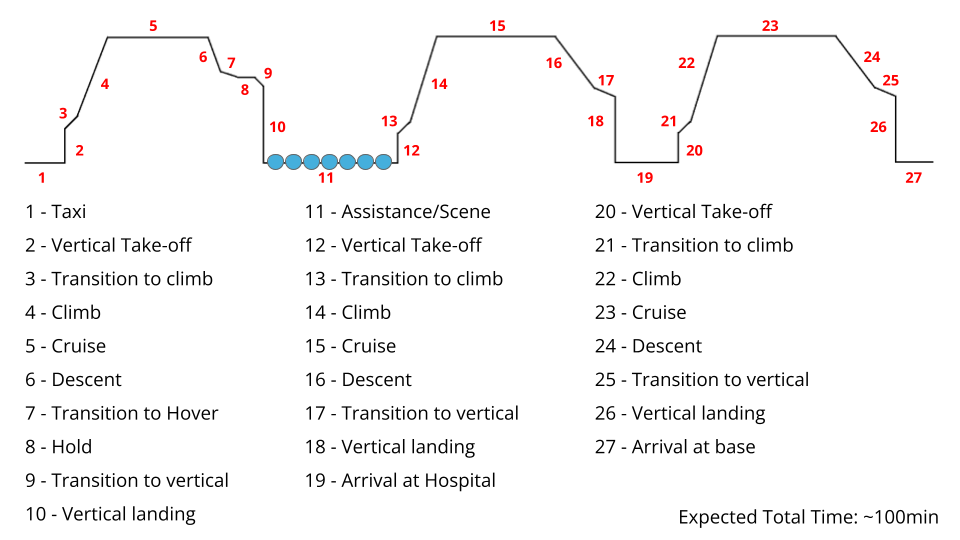
\includegraphics[width=\textwidth]{Imagens/PI - Semana 3.png}
    \caption{Missão}
    \label{fig:my_label}
\end{figure}
\FloatBarrier
O tempo foi estimado baseado em \textbf{who the fuck knows; inserir processo e citações}.\par
É importante mencionar que existe uma secção de Procura, secção 8, de forma a identificar o local onde a emergência toma lugar. Esta deverá ser entendida como voar a baixa altitude a menor velocidade do que aquela de cruise. É conceptualizada, também, como um voo com os rotores tilted com o ângulo de melhor eficiência. Este troço traz uma restrição ao design point (W/P, W/S) na forma de um teto máximo, sendo tanto maior quanto a velocidade. Foi entendido, duas semanas após esta, que o programa não conseguia simular esta manobra, devido à incapacidade de simular o forwards flight com tilted rotor, dando, por isso, uma restrição ao design space considerada excessiva e pouco realista.\par
{\Large{\textbf{Inserir aqui os dados todos deste json que estão no powerpoint}}}\par
As velocidades, os tempos e os ângulos foram estimadas baseado em {\large{\textbf{idfk,legit, fomos buscar isto onde}}}\par
\subsubsection{MTOW}
Para estimar o peso total da aeronave, foi tomados como dados históricos o peso do AW139, bem como o XV-15 {\large{\textbf{Imma be honest, eu não me lembro o que usamos como base, temos mesmo que ir ver}}}.\par
Dado, no entanto, o facto do programa discretizar a massa para cada componente, podemos usar apenas os dados antes mencionados para ter uma estimativa da massa total. Para obter a massa discretizada, foi necessário:
\begin{itemize}
    \item Estimar a massa de cada pessoa
    \item Estimar a massa do equipamento médico
    \item Estimar a proporção da massa de cada componente em relação à total
\end{itemize}
A massa de cada pessoa foi estimada em 100~kg, que é considerado uma estimativa conservativa e por cima. Foi baseado em {\large{\textbf{god knows where. and by god, I mean Joana, most likely}}}.\par
A massa do equipamento médico foi estimada com base em {\large{\textbf{god knows where. and by god, I mean Joana, most likely}}}.\par
A massa dos componentes da aeronave foi baseada no paper \cite{Bradley2015-yr}, em particular, na página 25, onde se encontra uma tabela, apresentada na figura \ref{sugartable}. Apesar de ser significamente diferente da nossa aeronave, foi considerado que era uma boa estimativa dos rácios de massa dum avião com configuração tube and wing, sendo por isso possível ajustar para o nosso design.\par
\FloatBarrier
\begin{figure}[h]
    \centering
    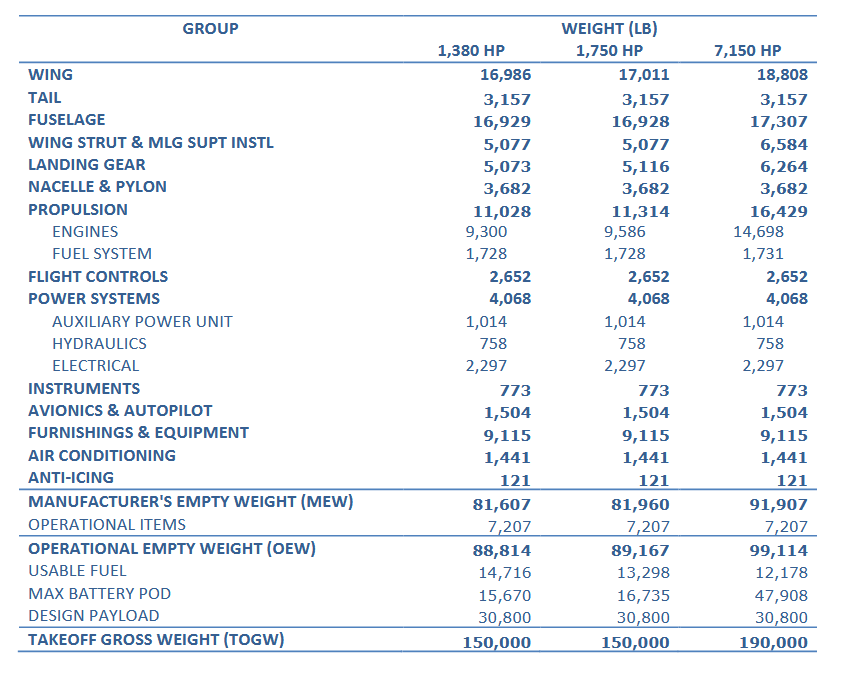
\includegraphics[width=\textwidth]{Imagens/boing sugar.PNG}
    \caption{Massa dos componentes do Boing SUGAR VOLT Source:\cite{Bradley2015-yr}}
    \label{sugartable}
\end{figure}
\FloatBarrier
Foi assumido uma relação linear, tal que a fração mássica fosse a mesma, ou aproximadamente igual, tanto no SUGAR VOLT como no nossa aeronave, no caso da estimação da massa das asas, cauda e fuselagem.\par
Dever-se-á notar que, nesta fase do projeto, não era sabido que o programa estimava o combustível e a massa das baterias, bem como que o VTOL era puramente a combustível. Devido a tal, foi estimada a massa de ambos baseado em dados históricos, nomeadamente, na percentagem da massa total que é do combustível.\textbf{Imma be honest, eu não sei onde fomos buscar os dados}\par
Abaixo, é apresentada a massa discretizada.\par
A altitude de cruise foi baseada na altitude mínima acima de zonas urbanas legislada pela FAA(?). \textbf{{\large{Quote, lol}}} Foi tido em conta que os helicópteros também conseguem voar a essa mesma altitutude \textbf{\large{{Quote, lol, AW139 deve ter uma altitude máxima de operaçao or something}}}
\FloatBarrier
\begin{table}[h]
\begin{tabular}{|l|l|}
\hline
Crew (100 kg/person)       & 200 kg                            \\ \hline
Passengers (100 kg/person) & 500 kg                            \\ \hline
Avionics                   & 24 kg                             \\ \hline
Payload Bay                & 200 kg (150 kg medical equipment) \\ \hline
Fuselage                   & 1200 kg                           \\ \hline
Main Wing                  & 840 kg                            \\ \hline
Horizontal Tail            & 100 kg                            \\ \hline
Vertical Tail              & 50 kg                             \\ \hline
Turboshaft -               & 462 kg                            \\ \hline
Battery                    & 200 kg                            \\ \hline
Generator                  & 462 kg                            \\ \hline
Electric Motor             & 510 kg                            \\ \hline
Fuel Tank                  & 1000 kg                           \\ \hline
\end{tabular}
\caption{Massa da aeronave discretizada - Semana 3}
\end{table}
\FloatBarrier
\subsubsection{Energy Network}
Tal como referido nas secções anteriores, foi escolhida uma arquitetura puramente turbo elétrica. Esta foi codificada no ficheiro json da seguinte forma:
\FloatBarrier
\begin{figure}[h]
    \centering
    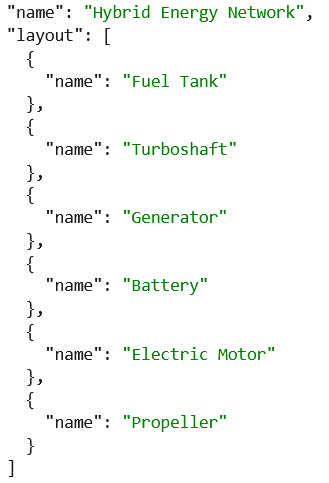
\includegraphics[width=0.4\textwidth]{Imagens/energy semana 3.png}
    \caption{Energy Network}
    \label{fig:my_label}
\end{figure}
\FloatBarrier
Esta configuração veio a ser considerada puramente conceptual devido a limitações do programa. A bateria teve que ser removida desta, posteriormente, devido ao facto do programa não simular recarregamento de baterias em voo. Também não era possível ligar a bateria e os motores elétricos em paralelo, dado que o programa só aceita arquiteturas sem ramos paralelos.\par
\section{Semana 4 - Design Point}
A semana quatro foi focada plenamente na procura dum design point válido.\par
Considere-se o Peso da aeronave projetada, W,a área de superfície da Asa, S, a Potência disponível, P, e a Área . A procura foi caracterizada por utilizar o programa disponibilizado e alterar os valores de forma a alterar os rácios: W/S, W/P e W/A. Desta forma, procurou-se encontrar um equilíbrio entre as dimensões da aeronave, a missão e os motores. Além de tal, teve-se em conta o grau de realismo dos valores ao se comparar com aqueles de aeronaves já concebidas, dado que o programa não consegue distinguir para casos irreais/contraditórios e que certos valores de diretamente relacionados com a performance são hardcoded no json, como o "power" dos motores elétricos.\par
\subsection{Descrição e Implementação}
É importante, primeiramente, dar uma breve descrição da aeronave, de forma a ser possível entender certas restrições tomadas, bem como esclarecer qual os cuidados tidos a implementá-la no programa.\par
\FloatBarrier
\begin{figure}[h]
    \centering
    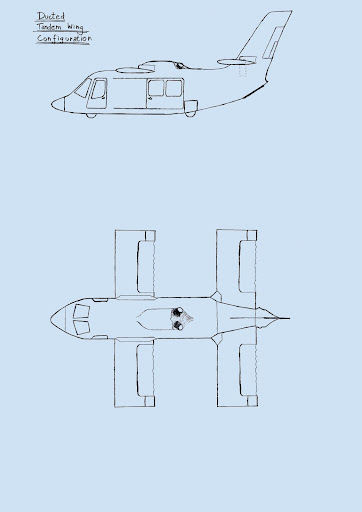
\includegraphics[width=0.4\textwidth]{Imagens/segundodesign2.jpg}
    \caption{Desgin escolhido}
    \label{designescolhido}
\end{figure}
\FloatBarrier
Baseado no AHP, foi escolhido o design apresentado em \ref{designescolhido}, em cima.\par
Este design apresenta tandem wing, com as asas desniveladas, de forma a diminuir a interferência. Nesta fase do design, o fator de interferência default no programa não foi mudado dada a ainda não realizada procura de relações empíricas. Além de tal, de forma a implementar a tandem wing, foi considerado que o o componente "Horizontal Tail" presente no ficheiro json de input para o programa poderia ser mudada de forma a ter a envergadura e corda necessário. Tal será mudado em futuras semanas, após ser descoberto como o programa calcula a área S e o lift nos cálculos de desempenho necessários para a estimação de combustível em cada troço, por análise direta do source code. A cauda de horizontal não é tratada como uma asa no código, não contribuindo para os cálculos do lift e do desempenho como se fosse uma asa principal, desprezando-se assim contribuíções que se tornam relevantes quando a as dimensões são comparáveis (neste caso iguais) às da asa principal.\par
Deve-se adicionar que as superfícies de controlo normalmente encontradas numa estabilizador horizontal encontram-se na asa posterior (de trás), utilizando-se, então, a configuração usual.\par
Em relação à propulsão, baseado no Lillium Jet, foi considerada uma distribuída, sobre a asa, no bordo de fuga. Esta é baseada em ter um motor com uma hélice cada ambos dentro de ductos convergentes. Não foi considerado utilizar um menor número de motores com maior potência, possivelmente colocados dentro da fuselagem, cada um alimentando várias hélices, dada a complexidade adicional na transmissão, que adiciona tanto peso como maior possibilidade de falha, É projetado, inicialmente, que existam cerca de 20 a 30 motores elétricos, dado que o Lillium Jet possui 36\cite{noauthor_2021-sz}. Diminuição do ruído, esteiras convergentes e os menores números de Mach locais devido aos ductos, o que permite maiores velocidades de rotação, (em comparação com sem ductos) são considerados como vantagens que deverão sobrepor-se ao atrito e ao peso impostos pela estrutura adicional necessária. Para ter estes em conta no programa, foi, nesta fase do projeto, apenas caracterizado os parâmetros já presentes no programa, nomeadamente, a quantidade, o raio, o número de pás, a velocidade, a massa, a eficiência e a potência. Tal foi devido a ser considerado que implementar um design mais realista só faria sentido numa fase mais avançada, nomeadamente, após se conseguir ter a versão simplificada a funcionar com valores plausiveis, dado que a tanto a procura de dados empíricos bem como a sua implementação no programa disponibilizado seria demorada e morosa e, por isso, demasiado custosa, dada a prioridades de ter um primeiro design funcional. É possível verificar a implementação escolhida em \ref{propulsoasemana4json}
\FloatBarrier
\begin{figure}[h]
    \centering
    \begin{subfigure}[h]{0.33\textwidth}
        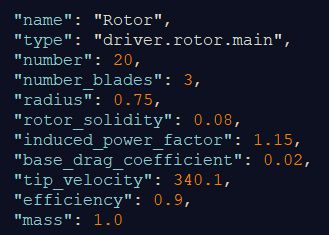
\includegraphics[width=\textwidth]{Imagens/rotor semana 4.PNG}
        \caption{Rotor - semana 4}
        \label{}
    \end{subfigure}
    \hfill
    \begin{subfigure}[h]{0.33\textwidth}
        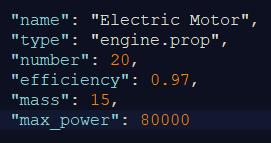
\includegraphics[width=\textwidth]{Imagens/motor semana 4.PNG}
        \caption{Motor elétrico - semana 4}
        \label{}
    \end{subfigure}
    \caption{Implementação da propulsão no ficheiro json - Semana 4}
    \label{propulsoasemana4json}
\end{figure}
\FloatBarrier
Esta escolha de arquitetura de propulsão impôs as seguintes restrições/decisões:
\begin{itemize}
    \item Os rotores deverão ter um diâmetro tal que a soma destes seja menor que a envergadura da asa (ou seja, que haja espaço para os acomodar)
    \item que a corda seja menor que o conjunto rotor + motor. Isto só pode ser tido em conta após ser escolhido o motor
    \item que a corda seja maior que a o diâmetro do rotor, de forma a que as proporções sejam plausíveis e não coloque problemas nem estruturais nem aerodinâmicos
    \item potência dos motores somados menor ou igual à gerada pelos gerados com o turboshaft
\end{itemize}
Para a estimar a massa e potência dos motores elétricos, foi tomada como referência o REB 90 ELECTRIC MOTOR da MGM COMPRO, dado o facto de ser utilizado em aeronáutica. A empresa afirma que é:"Highly variable and customizable, yet very powerful 80 KW electric motor. Suitable for a wide range of aviation projects, such as multirotor applications (UAVs), drones, gliders, as well as various types of marine projects. Tuned especially for complex projects with high demand for compact dimensions and very light weight.".\cite{noauthor_2021-ym}Este tinha 15kg e 80kW de potência\cite{noauthor_2021-ym}. Foi escolhido por ter sido considerado o melhor no mercado atual com as dimensões, tanto de volume como massa, e potência necessárias.\par
Além do descrito explicitamente aqui, este design em tudo se assemelha ao apresentado na semana 1, presente na figura \ref{DesingSketchini1}
\subsection{Design Point}
O Design Point da semana 4, uma primeira aproximação/estimação, foi conseguido ao preencher o json com os valores estimados e procurados iniciais e depois ajustar os valores de forma a conseguir um design considerado possível. Esta avaliação é conseguida com os rácios, já mencionados, W/S, W/P e W/A, e zonas nos gráficos (W/P, W/S) e (W/P,W/A) onde o design, segundo o modelo tomado, funcionaria em todos os troços. Será necessário mencionar, desde já, que apenas a massa total foi retirada do programa, e não a do combustível nem a da bateria nesta semana, devido a desconhecimento desta funcionalidade. Devido a tal, a exequibilidade da missão não foi tida em conta nesse campo, dado que, caso um troço não seja possível devido à mass fraction ter que ser maior que um (situação fisicamente impossível), o programa retorna um valor imaginário como massa de combustível ou de bateria; não retorna, no entanto, qualquer tipo de aviso. Tal é abordado numa semana mais adiante.\par
Este é caracterizado por:\par
\FloatBarrier
\begin{table}[h]
\begin{adjustbox}{width=1\textwidth}
\begin{tabular}{|l|l|lll}
\cline{1-2}
Crew (100 kg/person)       & 2 tripulantes - 200 kg                            &                       &                               &                                                                   \\ \cline{1-2} \cline{4-5} 
Passengers (100 kg/person) & 5 passageiros - 500 kg                            & \multicolumn{1}{l|}{} & \multicolumn{1}{l|}{Rotor}    & \multicolumn{1}{l|}{0 kg -2 rotores - 5 pás - 2 metros raio}      \\ \cline{1-2} \cline{4-5} 
Avionics                   & 24 kg                                             & \multicolumn{1}{l|}{} & \multicolumn{1}{l|}{Propeler} & \multicolumn{1}{l|}{50 kg -2 propelers - 4 pás - 2.3 metros raio} \\ \cline{1-2} \cline{4-5} 
Payload Bay                & 200 kg (150 kg medical equipment)                 & \multicolumn{1}{l|}{} & \multicolumn{1}{l|}{Gearbox}  & \multicolumn{1}{l|}{5 kg}                                         \\ \cline{1-2} \cline{4-5} 
Fuselage                   & 1200 kg - 4 metros comprimento - 1 metro diametro &                       &                               &                                                                   \\ \cline{1-2}
Main Wing                  & 840 kg - 7 aspect ratio - 3 metros corda          &                       &                               &                                                                   \\ \cline{1-2}
Horizontal Tail            & 100 kg - 5 aspect ratio - 0.5 metros corda        &                       &                               &                                                                   \\ \cline{1-2}
Vertical Tail              & 50 kg - 5 aspect ratio - 1 metro corda            &                       &                               &                                                                   \\ \cline{1-2}
Turboshaft -               & 0 kg - 210000kW                                   &                       &                               &                                                                   \\ \cline{1-2}
Battery                    & 200 kg - 360000 W/kg                              &                       &                               &                                                                   \\ \cline{1-2}
Generator                  & 924 kg                                            &                       &                               &                                                                   \\ \cline{1-2}
Electric Motor             & 510 kg - 200000W - 3 motores                      &                       &                               &                                                                   \\ \cline{1-2}
Fuel Tank                  & 1200 kg                                           &                       &                               &                                                                   \\ \cline{1-2}
\end{tabular}
\end{adjustbox}
\end{table}
\FloatBarrier
Dever-se-á notar os dados em falta, nomeadamente as massas. Certas massas foram incluídas noutros componetes, como, por exemplo: a massa dos dois turboshafts foi considerada no gerador. Outras, como a dos rotores, ficaram apenas por determinar, posteriormente. Dado a massa inicial de 1200 kg de fuselagem, foi considerado que poder-se-ia discritizar a massa para cada componente numa simulação posterior.\par
O resultado é apresentado de seguida:\par
\FloatBarrier
\begin{figure}[h]
    \centering
    \begin{subfigure}[h]{0.70\textwidth}
        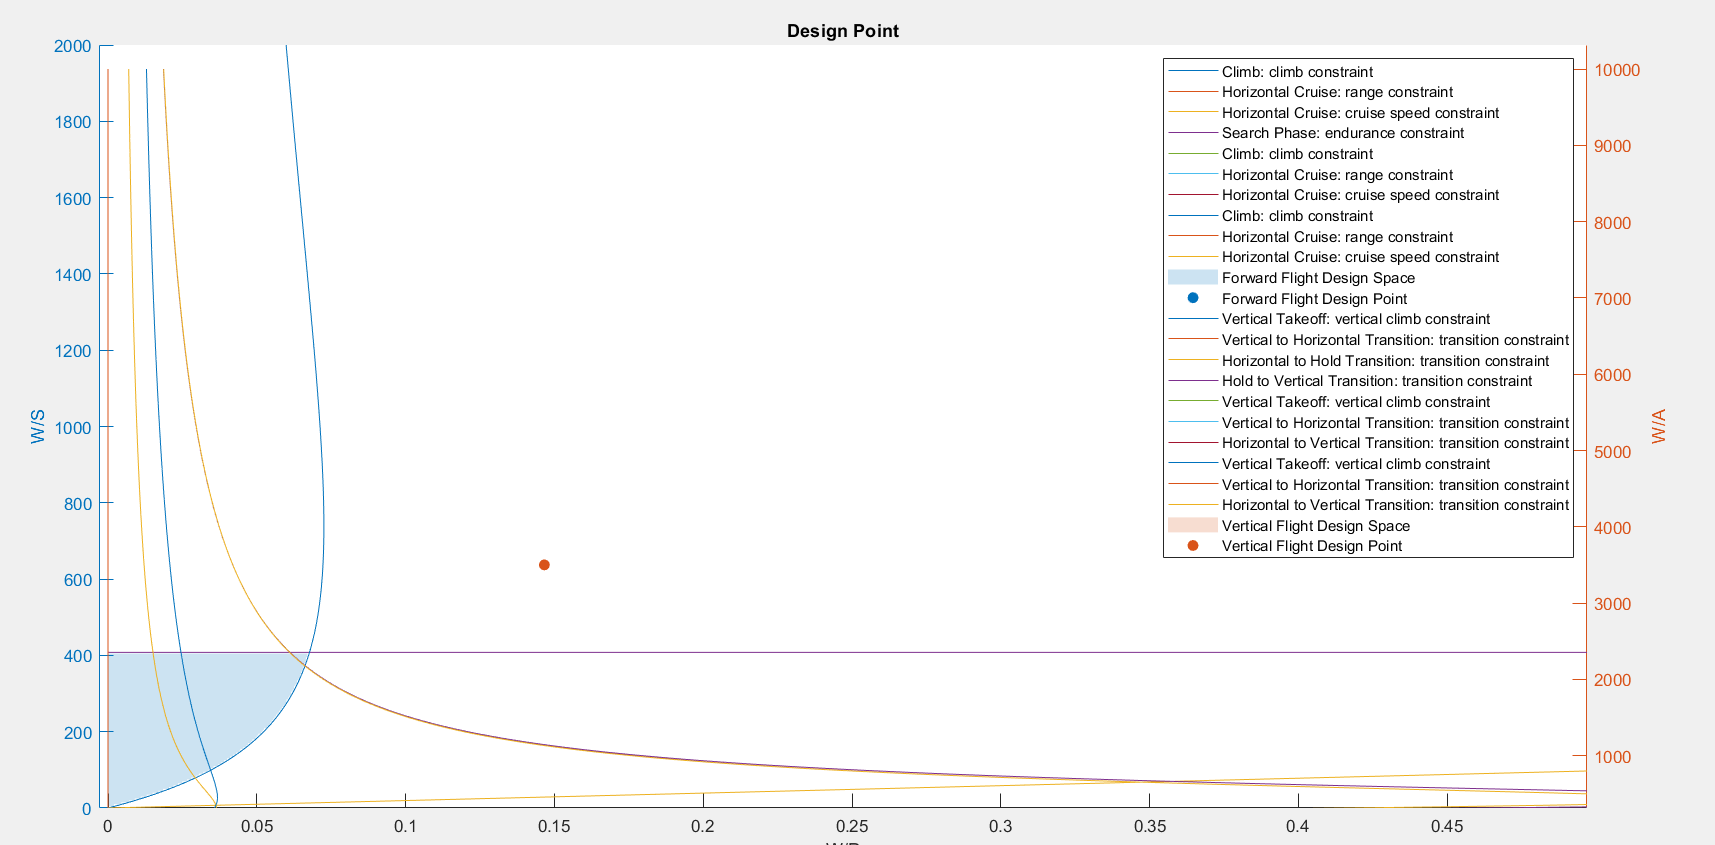
\includegraphics[width=\textwidth]{Imagens/firstplot_designpoint.PNG}
        \caption{Design Point}
        \label{}
    \end{subfigure}
    \hfill
    \begin{subfigure}[h]{0.70\textwidth}
        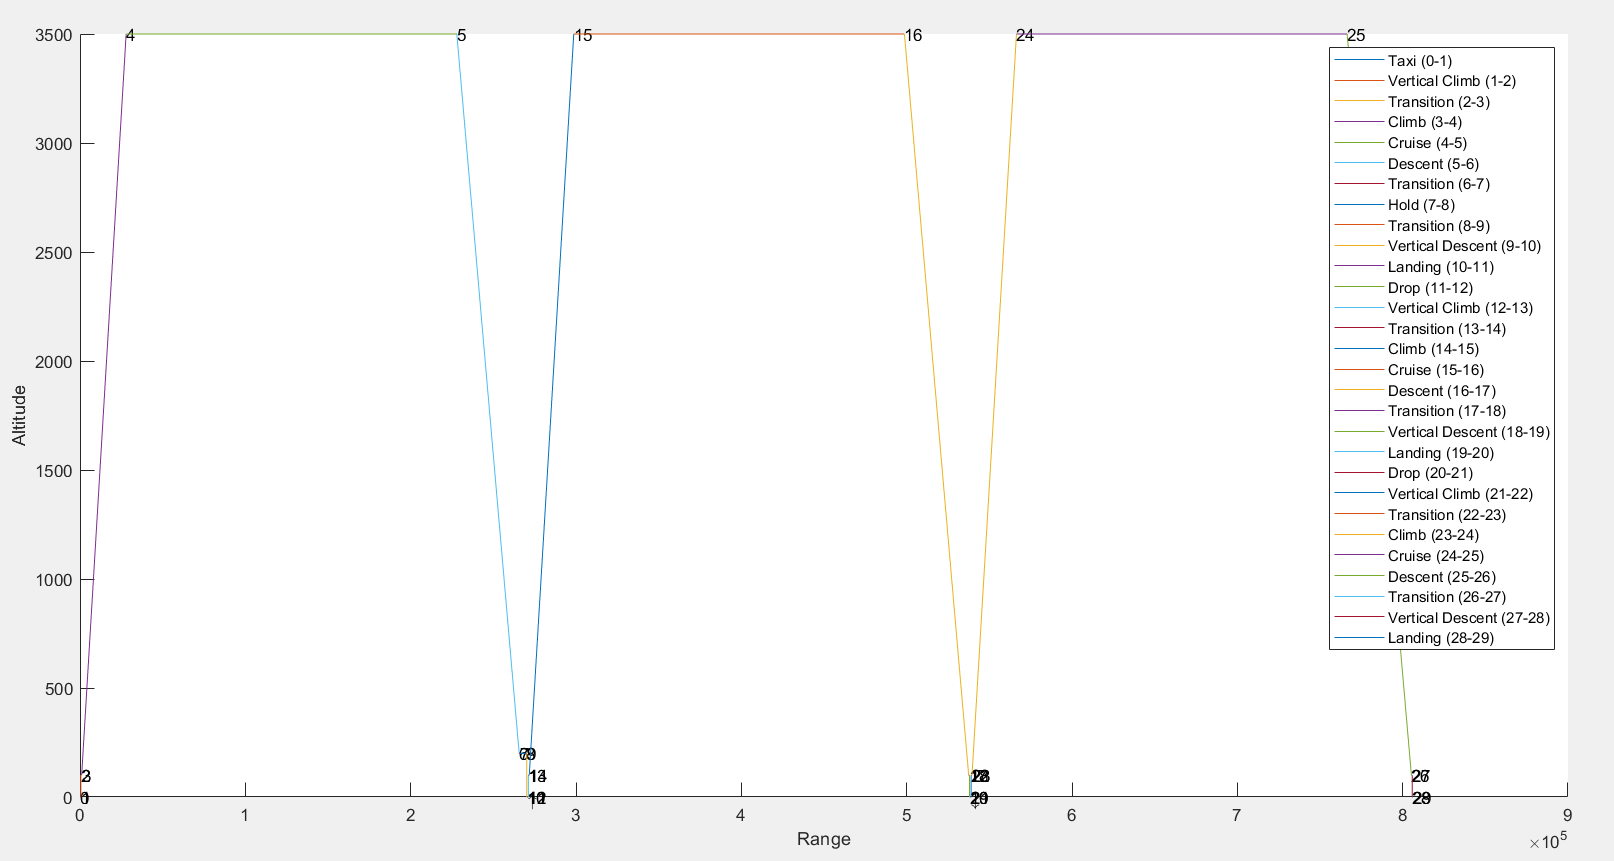
\includegraphics[width=\textwidth]{Imagens/firstplot_mission.PNG}
        \caption{Missão}
        \label{}
    \end{subfigure}
    \caption{Primeiro Plot gerado pelo programa}
    \label{firstplot}
\end{figure}
\FloatBarrier
Imediatamente, foi possível verificar dois aspetos: existem menos linhas no gráfico de design point que o número de troços; e a missão aparenta conter todos os troços corretamente. Esta ultíma afirmação é verdade.\par
Uma inspeção mais atenta, revelou que o menor número de linhas se deve não só a faltarem gráficos mas também a existirem linhas sobrepostas, ou quase sobrepostas, devido a existirem troços com as mesmas características.\par
Uma outra caracteristica importanto que foi logo notada é a de não ter sido formada área laranja, o que significava que existia uma falha na definição ou do veículo ou num troço vertical, não gerando linhas suficientes, dando erro, ou gerando uma na vertical que leva  a área laranja para zero.\par
O json foi alterado de forma a ter agora as seguintes características, mais credíveis:\par
\FloatBarrier 
 \begin{table}[h] 
 \begin{adjustbox}{width=1\textwidth} 
 \begin{tabular}{|c|c|c|c|}
 \hline 

\makecell{name: Crew ; \\ type: mass.point ; \\ mass: 200 ; \\ } & \makecell{name: Passengers ; \\ type: mass.point ; \\ mass: 500 ; \\ } & \makecell{name: Avionics ; \\ type: mass.point ; \\ mass: 5 ; \\ } & \makecell{name: Payload Bay ; \\ type: mass.point ; \\ mass: 10 ; \\ }\\ \hline \\ 
\makecell{name: Fuselage ; \\ type: fuselage ; \\ interf\_factor: 1.0 ; \\ diameter: 1.0 ; \\ length: 4.0 ; \\ mass: 800 ; \\ } & \makecell{name: Main Wing ; \\ type: wing.main ; \\ interf\_factor: 1.0 ; \\ aspect\_ratio: 7.0 ; \\ mean\_chord: 3.0 ; \\ oswald\_efficiency: 0.85 ; \\ airfoil:   type :  naca0012  \\   tc\_max : 0.15 \\   xc\_max : 0.3 \\   lift\_slope\_coefficient : 6.2 \\   cl\_max : 2.0  ; \\ sweep\_le: 10.0 ; \\ sweep\_c4: 15.0 ; \\ sweep\_tc\_max: 20.0 ; \\ mass: 200 ; \\ } & \makecell{name: Horizontal Tail ; \\ type: wing.htail ; \\ interf\_factor: 1.0 ; \\ aspect\_ratio: 5.0 ; \\ mean\_chord: 0.5 ; \\ oswald\_efficiency: 0.85 ; \\ airfoil:   type :  naca0012  \\   tc\_max : 0.15 \\   xc\_max : 0.3 \\   lift\_slope\_coefficient : 6.2 \\   cl\_max : 2.0  ; \\ sweep\_le: 10.0 ; \\ sweep\_c4: 15.0 ; \\ sweep\_tc\_max: 20.0 ; \\ mass: 50 ; \\ } & \makecell{name: Vertical Tail ; \\ type: wing.vtail ; \\ interf\_factor: 1.0 ; \\ aspect\_ratio: 5.0 ; \\ mean\_chord: 1.0 ; \\ oswald\_efficiency: 0.85 ; \\ airfoil:   type :  naca0012  \\   tc\_max : 0.15 \\   xc\_max : 0.3 \\   lift\_slope\_coefficient : 6.2 \\   cl\_max : 2.0  ; \\ sweep\_le: 10.0 ; \\ sweep\_c4: 15.0 ; \\ sweep\_tc\_max: 20.0 ; \\ mass: 50 ; \\ }\\ \hline \\ 
\makecell{name: Turboshaft ; \\ type: engine.prop ; \\ efficiency: 0.8 ; \\ mass: 100 ; \\ max\_power: 210000 ; \\ } & \makecell{name: 4-stroke Piston Engine ; \\ type: engine.prop ; \\ efficiency: 0.8 ; \\ mass: 100 ; \\ max\_power: 200000 ; \\ } & \makecell{name: Jet Engine ; \\ type: engine.jet ; \\ mass: 200 ; \\ max\_power: 120000 ; \\ } & \makecell{name: Battery ; \\ type: energy.electric ; \\ specific\_energy: 360000.0 ; \\ efficiency: 0.9 ; \\ reserve: 0.2 ; \\ mass: 0 ; \\ }\\ \hline \\ 
\makecell{name: Fuel Tank ; \\ type: energy.fuel ; \\ reserve: 0.06 ; \\ mass: 0 ; \\ } & \makecell{name: Rotor ; \\ type: driver.rotor.main ; \\ number: 2 ; \\ number\_blades: 5 ; \\ radius: 2 ; \\ rotor\_solidity: 0.08 ; \\ induced\_power\_factor: 1.15 ; \\ base\_drag\_coefficient: 0.02 ; \\ tip\_velocity: 240.1 ; \\ efficiency: 0.6 ; \\ mass: 20 ; \\ } & \makecell{name: Propeller ; \\ type: driver.rotor ; \\ number: 2 ; \\ number\_blades: 4 ; \\ radius: 2.3 ; \\ tip\_velocity: 240.1 ; \\ efficiency: 0.6 ; \\ mass: 10 ; \\ } & \makecell{name: Gearbox ; \\ type: gearbox ; \\ efficiency: 0.95 ; \\ mass: 5 ; \\ }\\ \hline \\ 
\makecell{name: Generator ; \\ type: generator ; \\ efficiency: 0.96 ; \\ mass: 50 ; \\ } & \makecell{name: Electric Motor ; \\ type: engine.prop ; \\ number: 3 ; \\ efficiency: 0.97 ; \\ mass: 50 ; \\ max\_power: 200000 ; \\ } &  & \\ \hline \\ 
\end{tabular} 
 \end{adjustbox} 
 \end{table} 
 \FloatBarrier 
\FloatBarrier 
 \begin{table}[h] 
 \begin{adjustbox}{width=1\textwidth} 
 \begin{tabular}{|c|c|c|}
 \hline 

\makecell{name: Taxi at Hospital ; \\ type: taxi ; \\ energy\_network: Hybrid Energy Network ; \\ time: 120 ; \\ altitude: 0 ; \\ } & \makecell{name: Vertical Takeoff ; \\ type: vertical\_climb ; \\ energy\_network: Electric Energy Network @ vertical flight ; \\ velocity: 8 ; \\ altitude: [0, 100] ; \\ } & \makecell{name: Vertical to Horizontal Transition ; \\ type: transition ; \\ energy\_network: Hybrid Energy Network ; \\ altitude: 100 ; \\ transition\_angle: 0 ; \\ time: 12 ; \\ velocity: [0, 16] ; \\ }\\ \hline \\ 
\makecell{name: Climb ; \\ type: climb ; \\ energy\_network: Hybrid Energy Network ; \\ velocity: 40 ; \\ altitude: [100, 3500] ; \\ angle: 7.2 ; \\ } & \makecell{name: Horizontal Cruise ; \\ type: cruise ; \\ energy\_network: Hybrid Energy Network ; \\ velocity: 120 ; \\ range: 200000 ; \\ altitude: 3500 ; \\ } & \makecell{name: Approach ; \\ type: descent ; \\ energy\_network: Hybrid Energy Network ; \\ velocity: -40 ; \\ altitude: [3500, 200] ; \\ angle: -5 ; \\ }\\ \hline \\ 
\makecell{name: Horizontal to Hold Transition ; \\ type: transition ; \\ energy\_network: Hybrid Energy Network ; \\ altitude: 200 ; \\ transition\_angle: 40 ; \\ time: 6 ; \\ velocity: [0, 30] ; \\ } & \makecell{name: Search Phase ; \\ type: hold ; \\ energy\_network: Hybrid Energy Network ; \\ velocity: 30 ; \\ time: 120 ; \\ altitude: 200 ; \\ } & \makecell{name: Hold to Vertical Transition ; \\ type: transition ; \\ energy\_network: Hybrid Energy Network ; \\ altitude: 200 ; \\ transition\_angle: 90 ; \\ time: 6 ; \\ velocity: [30, 0] ; \\ }\\ \hline \\ 
\makecell{name: Vertical Landing at Site ; \\ type: vertical\_descent ; \\ energy\_network: Electric Energy Network @ vertical flight ; \\ velocity: -6 ; \\ altitude: [200, 0] ; \\ } & \makecell{name: Passenger Tending For Pickup ; \\ type: landing ; \\ energy\_network: Hybrid Energy Network ; \\ time: 1800 ; \\ altitude: 0 ; \\ } & \makecell{name: Passenger Collection ; \\ type: load\_step ; \\ mass: 100 ; \\ time: 0 ; \\ altitude: 0 ; \\ }\\ \hline \\ 
\makecell{name: Vertical Takeoff ; \\ type: vertical\_climb ; \\ energy\_network: Electric Energy Network @ vertical flight ; \\ velocity: 8 ; \\ altitude: [0, 100] ; \\ } & \makecell{name: Vertical to Horizontal Transition ; \\ type: transition ; \\ energy\_network: Hybrid Energy Network ; \\ altitude: 100 ; \\ transition\_angle: 0 ; \\ time: 12 ; \\ velocity: [0, 16] ; \\ } & \makecell{name: Climb ; \\ type: climb ; \\ energy\_network: Hybrid Energy Network ; \\ velocity: 40 ; \\ altitude: [100, 3500] ; \\ angle: 7.2 ; \\ }\\ \hline \\ 
\makecell{name: Horizontal Cruise ; \\ type: cruise ; \\ energy\_network: Hybrid Energy Network ; \\ velocity: 120 ; \\ range: 200000 ; \\ altitude: 3500 ; \\ } & \makecell{name: Approach ; \\ type: descent ; \\ energy\_network: Hybrid Energy Network ; \\ velocity: -40 ; \\ altitude: [3500, 100] ; \\ angle: -5 ; \\ } & \makecell{name: Horizontal to Vertical Transition ; \\ type: transition ; \\ energy\_network: Hybrid Energy Network ; \\ altitude: 100 ; \\ transition\_angle: 90 ; \\ time: 12 ; \\ velocity: [40, 0] ; \\ }\\ \hline \\ 
\makecell{name: Vertical Landing at Hospital ; \\ type: vertical\_descent ; \\ energy\_network: Electric Energy Network @ vertical flight ; \\ velocity: -6 ; \\ altitude: [100, 0] ; \\ } & \makecell{name: Passenger Tending For Unloading ; \\ type: landing ; \\ energy\_network: Hybrid Energy Network ; \\ time: 550 ; \\ altitude: 0 ; \\ } & \makecell{name: Passenger Unloading Step ; \\ type: load\_step ; \\ mass: -100 ; \\ time: 0 ; \\ altitude: 0 ; \\ }\\ \hline \\ 
\makecell{name: Vertical Takeoff ; \\ type: vertical\_climb ; \\ energy\_network: Electric Energy Network @ vertical flight ; \\ velocity: 8 ; \\ altitude: [0, 100] ; \\ } & \makecell{name: Vertical to Horizontal Transition ; \\ type: transition ; \\ energy\_network: Hybrid Energy Network ; \\ altitude: 100 ; \\ transition\_angle: 0 ; \\ time: 12 ; \\ velocity: [0, 16] ; \\ } & \makecell{name: Climb ; \\ type: climb ; \\ energy\_network: Hybrid Energy Network ; \\ velocity: 40 ; \\ altitude: [100, 3500] ; \\ angle: 7.2 ; \\ }\\ \hline \\ 
\makecell{name: Horizontal Cruise ; \\ type: cruise ; \\ energy\_network: Hybrid Energy Network ; \\ velocity: 120 ; \\ range: 200000 ; \\ altitude: 3500 ; \\ } & \makecell{name: Approach ; \\ type: descent ; \\ energy\_network: Hybrid Energy Network ; \\ velocity: -40 ; \\ altitude: [3500, 100] ; \\ angle: -5 ; \\ } & \makecell{name: Horizontal to Vertical Transition ; \\ type: transition ; \\ energy\_network: Hybrid Energy Network ; \\ altitude: 100 ; \\ transition\_angle: 90 ; \\ time: 12 ; \\ velocity: [40, 0] ; \\ }\\ \hline \\ 
\makecell{name: Vertical Landing at Base ; \\ type: vertical\_descent ; \\ energy\_network: Electric Energy Network @ vertical flight ; \\ velocity: -6 ; \\ altitude: [100, 0] ; \\ } & \makecell{name: Final Post Landing Checkups ; \\ type: landing ; \\ energy\_network: Hybrid Energy Network ; \\ time: 120 ; \\ altitude: 0 ; \\ } & \\ \hline \\ 
\end{tabular} 
 \end{adjustbox} 
 \end{table} 
 \FloatBarrier 

Estes dados deram os seguintes plots:\par
\FloatBarrier
\begin{figure}[h]
    \centering
    \begin{subfigure}[h]{0.70\textwidth}
        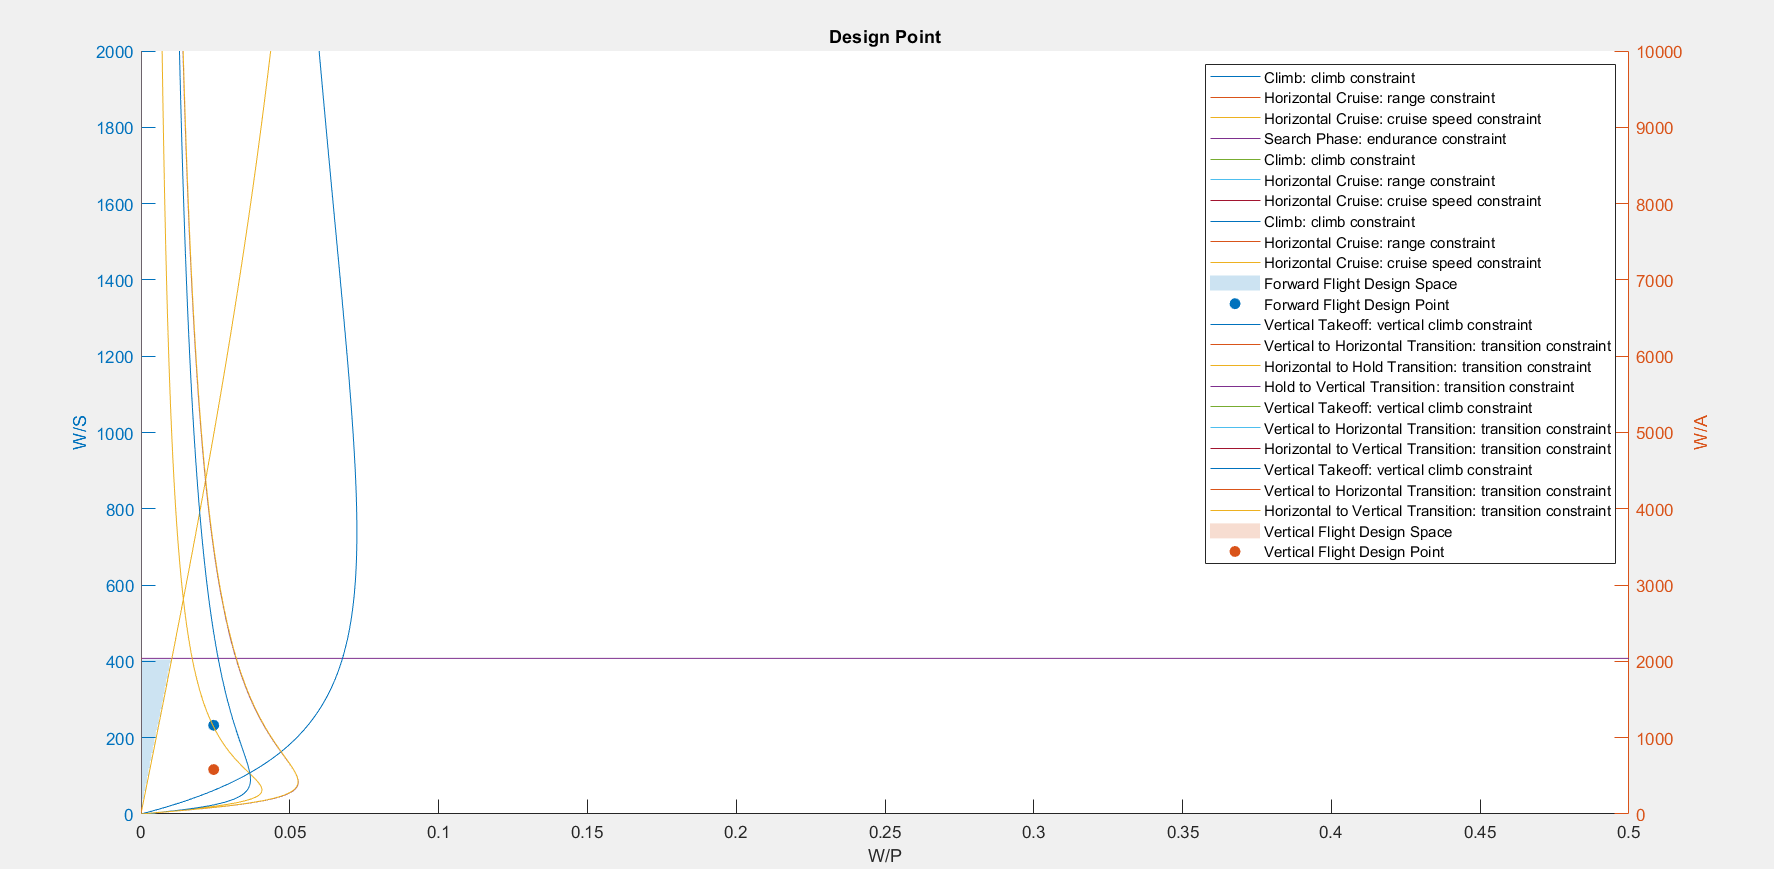
\includegraphics[width=\textwidth]{Imagens/secondplot_designpoint.PNG}
        \caption{Design Point}
        \label{}
    \end{subfigure}
    \hfill
    \begin{subfigure}[h]{0.70\textwidth}
        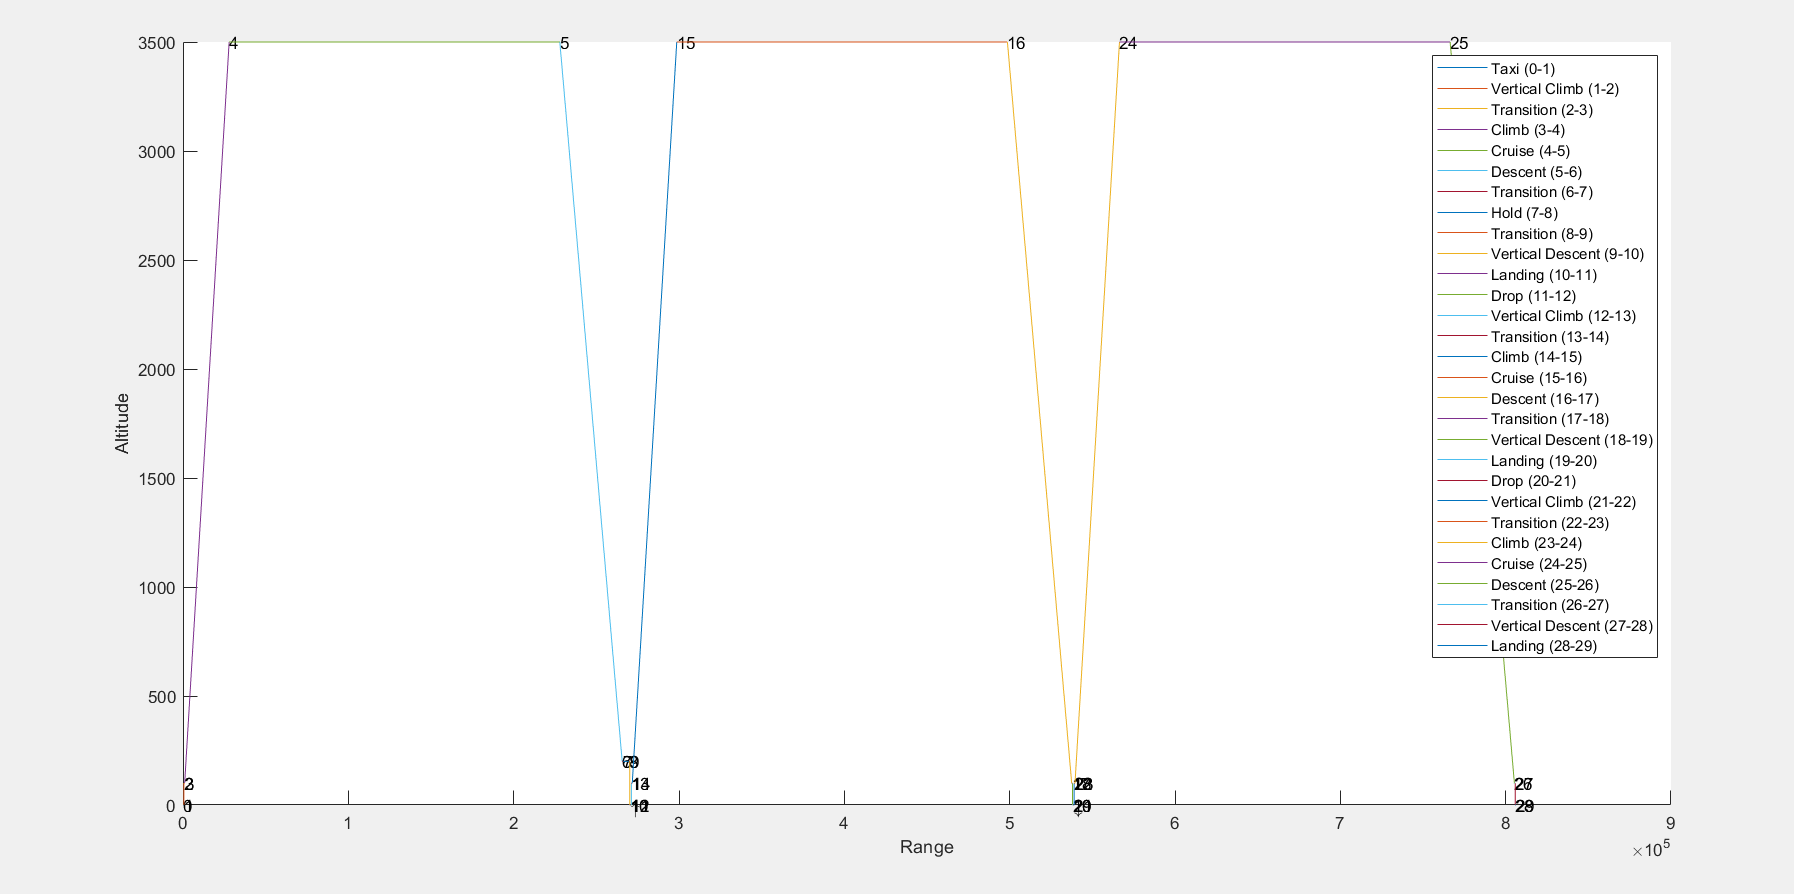
\includegraphics[width=\textwidth]{Imagens/secondplot_misson.PNG}
        \caption{Missão}
        \label{}
    \end{subfigure}
    \caption{Segundo Plot gerado pelo programa}
    \label{firstplot}
\end{figure}
\FloatBarrier
Este foi considerado uma melhor que o anterior, dado a presença de mais linhas, indicado a correção dum erro, bem como a valores de W/P mais perto da origem, ou seja, menores, para ambos os pontos. Isto significa que foi conseguido um compromisso onde é conseguido maior potência com menor peso.\par
É de notar que, no ficheiro json, as energy networks foram alteradas de forma a estarem devidamente formatadas. A "Hybrid Energy Network" foi a que sofreu maiores alterações. Primeiramente, foi adicionado ao turboshaft "brake\_specific\_fuel\_consumption", dado que o matlab o pedia; foi utilizado o valor default do programa. É importante, desde já, informar que este valor está errado, segundo valores históricos. Esta informação é explicitada e justificada devidamente na secção referente à semana 7, dado que só aí foi descoberto que o valor default estava em unidades imperiais e não SI. Segundamente, foi utilizado propellers como fim desta network, sendo-lhes adicionado: rotor\_solidity, base\_drag\_coefficient e induced\_power\_factor. É de notar que nos ficheiros json, estes valores estão apenas presentes nos rotores, e não nas propelles e que o programa esperara o uso de rotores em certos troços onde esta network foi utilizada, o que explica a necessidade de adicionar estes parâmetros. As propellers foram substituídas por rotores numa próxima semana. Notar que tal deveu-se tanto ao desconhecimento da nossa parte por a terminologia utilizada, dada nunca ter sido antes utilizada, bem como da falta de documentação do programa.\par
É apresentado de seguida a tabela com os dados colocados no json, estando todos estes em SI.\par
\FloatBarrier 
 \begin{table}[h] 
 \begin{adjustbox}{width=1\textwidth} 
 \begin{tabular}{|c|c|c|c|}
 \hline 

\makecell{name: Crew ; \\ type: mass.point ; \\ mass: 200 ; \\ } & \makecell{name: Passengers ; \\ type: mass.point ; \\ mass: 500 ; \\ } & \makecell{name: Avionics ; \\ type: mass.point ; \\ mass: 5 ; \\ } & \makecell{name: Payload Bay ; \\ type: mass.point ; \\ mass: 10 ; \\ }\\ \hline \\ 
\makecell{name: Fuselage ; \\ type: fuselage ; \\ interf\_factor: 1.0 ; \\ diameter: 1.0 ; \\ length: 4.0 ; \\ mass: 800 ; \\ } & \makecell{name: Main Wing ; \\ type: wing.main ; \\ interf\_factor: 1.0 ; \\ aspect\_ratio: 7.0 ; \\ mean\_chord: 3.0 ; \\ oswald\_efficiency: 0.85 ; \\ airfoil:   type :  naca0012  \\   tc\_max : 0.15 \\   xc\_max : 0.3 \\   lift\_slope\_coefficient : 6.2 \\   cl\_max : 2.0  ; \\ sweep\_le: 10.0 ; \\ sweep\_c4: 15.0 ; \\ sweep\_tc\_max: 20.0 ; \\ mass: 200 ; \\ } & \makecell{name: Horizontal Tail ; \\ type: wing.htail ; \\ interf\_factor: 1.0 ; \\ aspect\_ratio: 5.0 ; \\ mean\_chord: 0.5 ; \\ oswald\_efficiency: 0.85 ; \\ airfoil:   type :  naca0012  \\   tc\_max : 0.15 \\   xc\_max : 0.3 \\   lift\_slope\_coefficient : 6.2 \\   cl\_max : 2.0  ; \\ sweep\_le: 10.0 ; \\ sweep\_c4: 15.0 ; \\ sweep\_tc\_max: 20.0 ; \\ mass: 50 ; \\ } & \makecell{name: Vertical Tail ; \\ type: wing.vtail ; \\ interf\_factor: 1.0 ; \\ aspect\_ratio: 5.0 ; \\ mean\_chord: 1.0 ; \\ oswald\_efficiency: 0.85 ; \\ airfoil:   type :  naca0012  \\   tc\_max : 0.15 \\   xc\_max : 0.3 \\   lift\_slope\_coefficient : 6.2 \\   cl\_max : 2.0  ; \\ sweep\_le: 10.0 ; \\ sweep\_c4: 15.0 ; \\ sweep\_tc\_max: 20.0 ; \\ mass: 50 ; \\ }\\ \hline \\ 
\makecell{name: Turboshaft ; \\ type: engine.prop ; \\ efficiency: 0.8 ; \\ mass: 100 ; \\ max\_power: 210000 ; \\ } & \makecell{name: 4-stroke Piston Engine ; \\ type: engine.prop ; \\ efficiency: 0.8 ; \\ mass: 100 ; \\ max\_power: 200000 ; \\ } & \makecell{name: Jet Engine ; \\ type: engine.jet ; \\ mass: 200 ; \\ max\_power: 120000 ; \\ } & \makecell{name: Battery ; \\ type: energy.electric ; \\ specific\_energy: 360000.0 ; \\ efficiency: 0.9 ; \\ reserve: 0.2 ; \\ mass: 0 ; \\ }\\ \hline \\ 
\makecell{name: Fuel Tank ; \\ type: energy.fuel ; \\ reserve: 0.06 ; \\ mass: 0 ; \\ } & \makecell{name: Rotor ; \\ type: driver.rotor.main ; \\ number: 2 ; \\ number\_blades: 5 ; \\ radius: 2 ; \\ rotor\_solidity: 0.08 ; \\ induced\_power\_factor: 1.15 ; \\ base\_drag\_coefficient: 0.02 ; \\ tip\_velocity: 240.1 ; \\ efficiency: 0.6 ; \\ mass: 20 ; \\ } & \makecell{name: Propeller ; \\ type: driver.rotor ; \\ number: 2 ; \\ number\_blades: 4 ; \\ radius: 2.3 ; \\ tip\_velocity: 240.1 ; \\ efficiency: 0.6 ; \\ mass: 10 ; \\ } & \makecell{name: Gearbox ; \\ type: gearbox ; \\ efficiency: 0.95 ; \\ mass: 5 ; \\ }\\ \hline \\ 
\makecell{name: Generator ; \\ type: generator ; \\ efficiency: 0.96 ; \\ mass: 50 ; \\ } & \makecell{name: Electric Motor ; \\ type: engine.prop ; \\ number: 3 ; \\ efficiency: 0.97 ; \\ mass: 50 ; \\ max\_power: 200000 ; \\ } &  & \\ \hline \\ 
\end{tabular} 
 \end{adjustbox} 
 \end{table} 
 \FloatBarrier 


\par
O design apresentado acima, apesar de se apresentar como uma primeira base sólida, teve três problemas, ambos na missão: valores errados/irrealistas na missão; fases de missão erradas; e o uso de energy networks não suportadas.\par
O primeiro é caracterizado pelo o uso de velocidades demasiado elevadas, bem como de transition angles errados (devido a desconhecimento de como o programa interpretava esta valor). Além de tal, a search fase foi entendida como incorretamente caracterizada. Esta era descrita no json como uma hold, ou seja, voar a velocidade abaixo da de cruise, e foi visionada como a aeronave a voar a baixa velocidade com os motores tilted no ângulo mais efficiente, sendo, assim, mais efficiente que um simples hover dado a sustentação adicional dada pelas asas. No entanto, o programa entende que apenas a sustentação das asas é importante para neste mode de operação, pelo que é necessária uma velocidade alta para não entrar em stall. Isto é traduzido no programa como a existência duma linha vertical no plot do design point (W/S,W/A) baixa, reduzindo largamente a área. De forma a corrigir isto e gerar valores mais realista, foi mudado para hover. Entendemos este modo como uma estimativa conservativa, dada que a search phase pode ser realizada como anteriormente visionada na mesma, sendo, na realidade, mais eficiente que um simpls hover; ou seja, a limitação imposta pelo hover continua a ser maior que a real. Estas mudanças podem ser sumarizadas por:\par
\begin{itemize}
    \item Vertical take off velocity: 4 m/s
    \item Transition: 45º
    \item Hold changed to hover for search phase
    \item Search phase: 35 m/s
    \item Cruise velocity: 98 m/s
\end{itemize}
Por útlimo, vertical take off and landing não é suportado com combustível. Era assumido, no desenvolvimento projeto até aqui, dada a existência de múltiplos veículos capazes de realizar uma descolagem/aterragem com combustível, que este seria suportado no programa. É devido a tal que nunca se falou de descolagens verticais com baterias. No entanto, dada a falta de estimativas empíricas para fix wing aircraft presentes na literatura, não só não está presente no programa, como não foi possível implementá-la. Tal foi discutido com um dos criadores do programa, numa chamada por zoom de uma hora, numa tentativa de entender o que o programa suporta e quais a soluções possíveis. Foi-nos recomendados ceder ao uso de baterias ou encontrar relações empíricas, sendo-nos oferecida ajuda para serem implementadas. Dado que a nossa procura, ao longo da semana, foi infrutífera, escolhemos, reiterando, usar baterias.\par
Com estas mudanças, foi conseguido o seguinte design point:
\FloatBarrier
\begin{figure}[h]
    \centering
    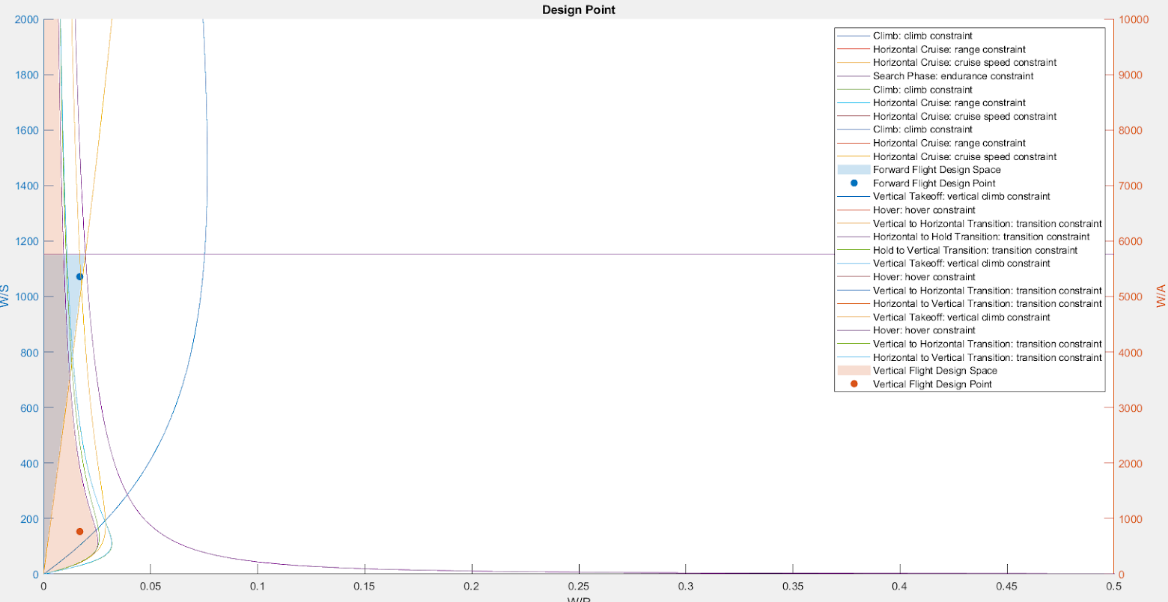
\includegraphics[width=\textwidth]{Imagens/semana4 powerpoint designpoint.png}
    \caption{Desgin Point final semanal- Semana 4}
    \label{designescolhido}
\end{figure}
\FloatBarrier
{\large\textbf{Colocar designs intermedios e tal; esta semana foi um inferno e precisamos de transmitir isso bem}}
\section{Semana 5 e 6 - Design Point+Wing\&Tail+Engine Selection}
\subsection{Introdução}
Esta secção apresenta os desenvolvimentos durante as semanas 5 e 6. Dada a falta duma reunião de acompanhamento na semana 5, devido a \textbf{??friado or something??}, o trabalho foi realizado continuamente ao longo destas duas semanas, sendo, por isso, amalgamadas numa única secção.\par
O Design Point foi o principal aspeto desenvolvido ao longo dessas duas semanas, sendo um trabalho contínuo. FOi conseguido um desgin satisfatório\par
A seleção da Wing\&Tail foi realizado por \textbf{inserir numero de membros} membros da equipa, sendo mais desenvolvido na semana 6. Foi conseguido um resultado satisfatório, mas os cálculos de desempempenho realizados pelo programa não ficaram ainda corrigidos totalmente para a escolha. Foi considerada uma estimativa conservadora.\par
O Engine Selection benefeciou do nosso estudo de mercado anterior e da tabela fornecido por o docente de motores disponiveis no mercado, tendo ocupado pouco tempo e obtido um resultado satisfatório.\par

\subsection{Desgin Point}
O Design Point foi novamente desenvolvido esta semana, revelando-se um trabalho moroso e demorado, tendo parte da equipa trabalhado exclusivamente neste, a fim de distribuir melhor o trabalho. O desenvolvimento foi feito por turnos, principal e inicialmente, a fim de cada um atacar o problema de ângulos diferentes. Este trabalho consistiu principalmente em ajustar os seguintes valores:
\begin{itemize}
    \item Wing Aspect Ratio
    \item Components Mass
    \item Mission Segment Range - principalmente o Cruise Range
    \item Mission Segment Velocity
    \item Mission Segment Altitude
\end{itemize}
Após trabalho individual, continuamente comunicado e partilhado com o resto do grupo, foi desenvolvido trabalho em conjunto a fim de partilhar e melhor afinar os ajustes, bem como detetar problemas adicionais.\par
No início da \textbf{sexta ou quinta semana?? acho que sexta}, segunda-feira, por análise do ficheiro adt.m, foi descoberto que existia um segundo parâmetro adicional, que podia ser chamado que fazia o programa escrever todos os resultados obtidos, bem como os hardcoded, num ficheiro json. Ao correr o programa com este parâmetro, um erro foi gerado no terminal, indicando que o ficheiro json não consegui ser gerado devido a tentar escrever um formato não suportado. Não era indicado pela mensagem, no entanto, que o que o impedia em concreto era a existência de um número complexo num dos dados. Por inspeção direta das variáveis geradas pelo programa, foi descoberto, que a massa da bateria e a massa do combustível eram imaginárias e que tal seria provavelmente a razão pela qual o json não era gerado. Foi teorizado, e dois dias depois confirmado pelos developers do programa, que a massa imaginária implicava que o avião não conseguia realizar o trajeto proposto. Concretamente, uma das mass fractions seria maior que um, o que revela um cenário impossível. Tal levou ao range ter que ser diminuído para cerca de 33km por cruise segment, havendo 3 no total, e impeliu uma procura por valores errados nas definições, dado que este range extremamente curto não era realista. Como termo de comparação de alcance, foi utilizado o AW 139, que tem um alcance máximo de 1032km.\par
Nessa mesma semana, quinta-feira, foi teorizado que o brake-specific fuel consumption estava errado, dado que era um dos valores default ainda não alterados e o único que não os das asas que nos parecesse alterar o consumo de combustível. Baseado em \textbf{{\Large Inserir citação que agr não sei onde está}}, concluímos que estava errado por duas ordens grandeza, o que indicaria que ou foi mal copiado ou estava escrito em unidades diferentes das SI. Após falar com um dos programadores do programa disponibilizado, concluiu-se que esse valor estava em unidades imperiais, apesar dos outros valores default estarem em SI, estando errada por duas ordens de grandeza.\par
Ao procurar corrigir valores antes de se mudar o brake specific fuel consumption, tentou-se conseguir o alcance máximo possível. Foi descoberto que valores perto de 35km para os três segmentos de cruise realizavam um perfil de missão possível. Ao ajustar o aspect ratio, conseguia-se alterar o valor máximo, mas sem ultrapassar muito este valor, situando-se no máximo a 40km. Escolheu-se optimizar, então, os cruise segments individualmente. Ao realizar tal, foi descoberto que o programa permitia ter um alcance infinito no último segmento de cruise, ou seja, no de retorno ao hospital. Era previsto, pelo programa, que seria possível voar na ordem milhões de kilometros, estimando um combustível necessário de 25kg. Após falar com um dos programadores, na mesma reunião que a suprareferida, foi concluído que havia um bug, consistindo em um das equações de desempenho estar a ser mal realizada. Foi-nos disponibilizada a versão sem erros, posteriormente.\par
É apresentado em baixo o gráfico do melhor design point obtido.
\FloatBarrier
\begin{figure}[h]
    \centering
    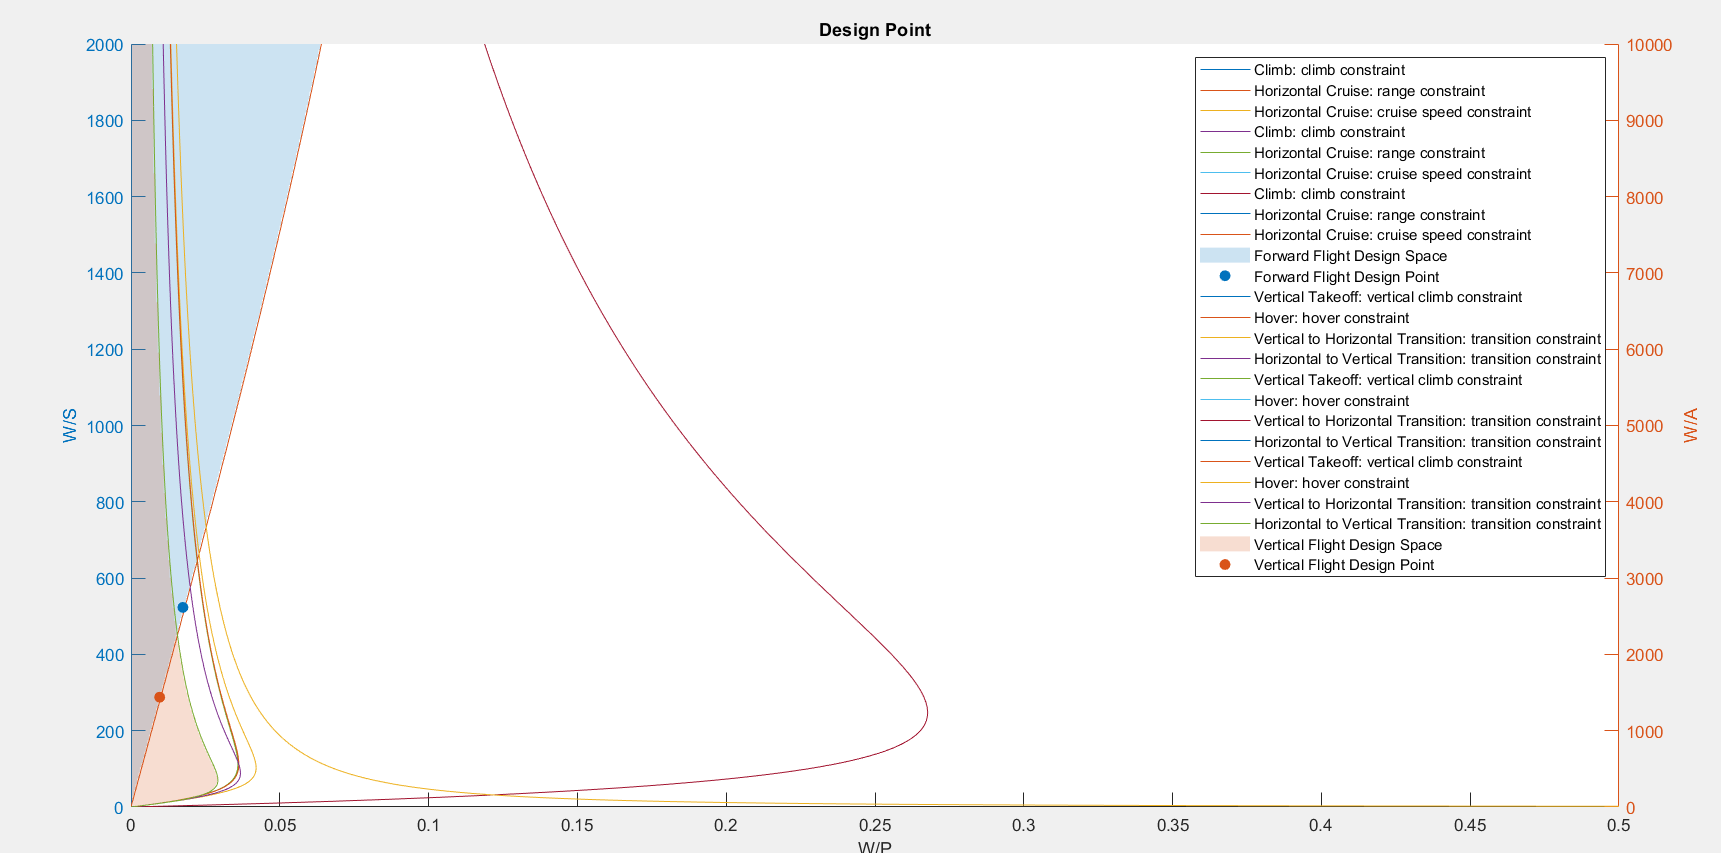
\includegraphics[width=\textwidth]{Imagens/semana6_com_brake_specific_incorreto_designpoint.PNG}
    \caption{Desgin Point com brake-specific fuel consumption incorreto e cerca de 35 km em cada cruise segment - Semana 6}
    \label{designpoint_plot_semana6_correto_specifc_fuel consumption}
\end{figure}
\FloatBarrier

Em baixo, é apresentada a tabela \ref{"tabela_wrong_fuel_consumption"}, onde se encontram os valores para a missão descrita no último design. Note-se os valores do alcance nos segmentos de cruise, uma menor altitude de cruise, bem como valores baixos para altitudes, velocidades e tempos nos outros segmentos em geral. Tal evidência as restrições que nos levaram a acreditar que um dos valores default haveria de estar errado.\par
\FloatBarrier 
 \begin{table}[h] 
 \begin{adjustbox}{width=1\textwidth} 
 \begin{tabular}{|c|c|c|}
 \hline 

\makecell{name: Taxi at Hospital ; \\ type: taxi ; \\ energy\_network: Hybrid Energy Network ; \\ time: 120 ; \\ altitude: 0 ; \\ } & \makecell{name: Vertical Takeoff ; \\ type: vertical\_climb ; \\ energy\_network: Electric Energy Network @ vertical flight ; \\ velocity: 3.5 ; \\ altitude: [0, 50] ; \\ } & \makecell{name: Hover ; \\ type: hover ; \\ energy\_network: Electric Energy Network @ vertical flight ; \\ altitude: 50.0 ; \\ time: 5 ; \\ }\\ \hline \\ 
\makecell{name: Vertical to Horizontal Transition ; \\ type: transition ; \\ energy\_network: Hybrid Energy Network ; \\ altitude: 50 ; \\ transition\_angle: 90 ; \\ time: 12 ; \\ velocity: [0, 16] ; \\ } & \makecell{name: Climb ; \\ type: climb ; \\ energy\_network: Hybrid Energy Network ; \\ velocity: 16 ; \\ altitude: [50, 2500] ; \\ angle: 7.2 ; \\ } & \makecell{name: Horizontal Cruise ; \\ type: cruise ; \\ energy\_network: Hybrid Energy Network @Cruise ; \\ velocity: 97 ; \\ range: 35000 ; \\ altitude: 2500 ; \\ }\\ \hline \\ 
\makecell{name: Approach ; \\ type: descent ; \\ energy\_network: Hybrid Energy Network ; \\ velocity: -20 ; \\ altitude: [2500, 50] ; \\ angle: -7 ; \\ } & \makecell{name: Horizontal to Vertical Transition ; \\ type: transition ; \\ energy\_network: Hybrid Energy Network ; \\ altitude: 50 ; \\ transition\_angle: 40 ; \\ time: 12 ; \\ velocity: [20, 0] ; \\ } & \makecell{name: Vertical Landing at Site ; \\ type: vertical\_descent ; \\ energy\_network: Electric Energy Network @ vertical flight ; \\ velocity: -4 ; \\ altitude: [50, 0] ; \\ }\\ \hline \\ 
\makecell{name: Passenger Tending For Pickup ; \\ type: landing ; \\ energy\_network: Hybrid Energy Network ; \\ time: 1800 ; \\ altitude: 0 ; \\ } & \makecell{name: Passenger Collection ; \\ type: load\_step ; \\ mass: 100 ; \\ time: 0 ; \\ altitude: 0 ; \\ } & \makecell{name: Vertical Takeoff ; \\ type: vertical\_climb ; \\ energy\_network: Electric Energy Network @ vertical flight ; \\ velocity: 4 ; \\ altitude: [0, 50] ; \\ }\\ \hline \\ 
\makecell{name: Hover ; \\ type: hover ; \\ energy\_network: Electric Energy Network @ vertical flight ; \\ altitude: 50.0 ; \\ time: 5 ; \\ } & \makecell{name: Vertical to Horizontal Transition ; \\ type: transition ; \\ energy\_network: Hybrid Energy Network ; \\ altitude: 50 ; \\ transition\_angle: 60 ; \\ time: 12 ; \\ velocity: [0, 16] ; \\ } & \makecell{name: Climb ; \\ type: climb ; \\ energy\_network: Hybrid Energy Network ; \\ velocity: 16 ; \\ altitude: [50, 2500] ; \\ angle: 7.2 ; \\ }\\ \hline \\ 
\makecell{name: Horizontal Cruise ; \\ type: cruise ; \\ energy\_network: Hybrid Energy Network @Cruise ; \\ velocity: 97 ; \\ range: 150000 ; \\ altitude: 2500 ; \\ } & \makecell{name: Approach ; \\ type: descent ; \\ energy\_network: Hybrid Energy Network ; \\ velocity: -20 ; \\ altitude: [2500, 50] ; \\ angle: -7 ; \\ } & \makecell{name: Horizontal to Vertical Transition ; \\ type: transition ; \\ energy\_network: Hybrid Energy Network ; \\ altitude: 50 ; \\ transition\_angle: 40 ; \\ time: 12 ; \\ velocity: [20, 0] ; \\ }\\ \hline \\ 
\makecell{name: Vertical Landing at Hospital ; \\ type: vertical\_descent ; \\ energy\_network: Electric Energy Network @ vertical flight ; \\ velocity: -4 ; \\ altitude: [50, 0] ; \\ } & \makecell{name: Passenger Tending For Unloading ; \\ type: landing ; \\ energy\_network: Hybrid Energy Network ; \\ time: 550 ; \\ altitude: 0 ; \\ } & \makecell{name: Passenger Unloading Step ; \\ type: load\_step ; \\ mass: -100 ; \\ time: 0 ; \\ altitude: 0 ; \\ }\\ \hline \\ 
\makecell{name: Vertical Takeoff ; \\ type: vertical\_climb ; \\ energy\_network: Electric Energy Network @ vertical flight ; \\ velocity: 3.5 ; \\ altitude: [0, 50] ; \\ } & \makecell{name: Hover ; \\ type: hover ; \\ energy\_network: Electric Energy Network @ vertical flight ; \\ altitude: 50.0 ; \\ time: 5 ; \\ } & \makecell{name: Vertical to Horizontal Transition ; \\ type: transition ; \\ energy\_network: Hybrid Energy Network ; \\ altitude: 50 ; \\ transition\_angle: 60 ; \\ time: 12 ; \\ velocity: [0, 16] ; \\ }\\ \hline \\ 
\makecell{name: Climb ; \\ type: climb ; \\ energy\_network: Hybrid Energy Network ; \\ velocity: 16 ; \\ altitude: [50, 2500] ; \\ angle: 7.2 ; \\ } & \makecell{name: Horizontal Cruise ; \\ type: cruise ; \\ energy\_network: Hybrid Energy Network @Cruise ; \\ velocity: 97 ; \\ range: 999999999999999100000 ; \\ altitude: 2500 ; \\ } & \makecell{name: Approach ; \\ type: descent ; \\ energy\_network: Hybrid Energy Network ; \\ velocity: -20 ; \\ altitude: [2500, 50] ; \\ angle: -7 ; \\ }\\ \hline \\ 
\makecell{name: Horizontal to Vertical Transition ; \\ type: transition ; \\ energy\_network: Hybrid Energy Network ; \\ altitude: 50 ; \\ transition\_angle: 40 ; \\ time: 12 ; \\ velocity: [20, 0] ; \\ } & \makecell{name: Vertical Landing at Base ; \\ type: vertical\_descent ; \\ energy\_network: Electric Energy Network @ vertical flight ; \\ velocity: -4 ; \\ altitude: [50, 0] ; \\ } & \makecell{name: Final Post Landing Checkups ; \\ type: landing ; \\ energy\_network: Hybrid Energy Network ; \\ time: 120 ; \\ altitude: 0 ; \\ }\\ \hline \\ 
\end{tabular} 

 \caption{Caracterização dos segmentos de missão - semana 6, primeiro design com brake specific fuel consumption correto} \label{"tabela_wrong_fuel_consumption"}
 \end{adjustbox}
 \end{table} 
 \FloatBarrier 

Após corrigir o brake-specific fuel consumption, e ajustar o range para 200km por segmento de cruise, ficando com um alcance superior a 700km (600km de cruise + 100+ km de subida e descida na diagonal), obteve-se os seguintes resultados:
\FloatBarrier
\begin{figure}[h]
    \centering
    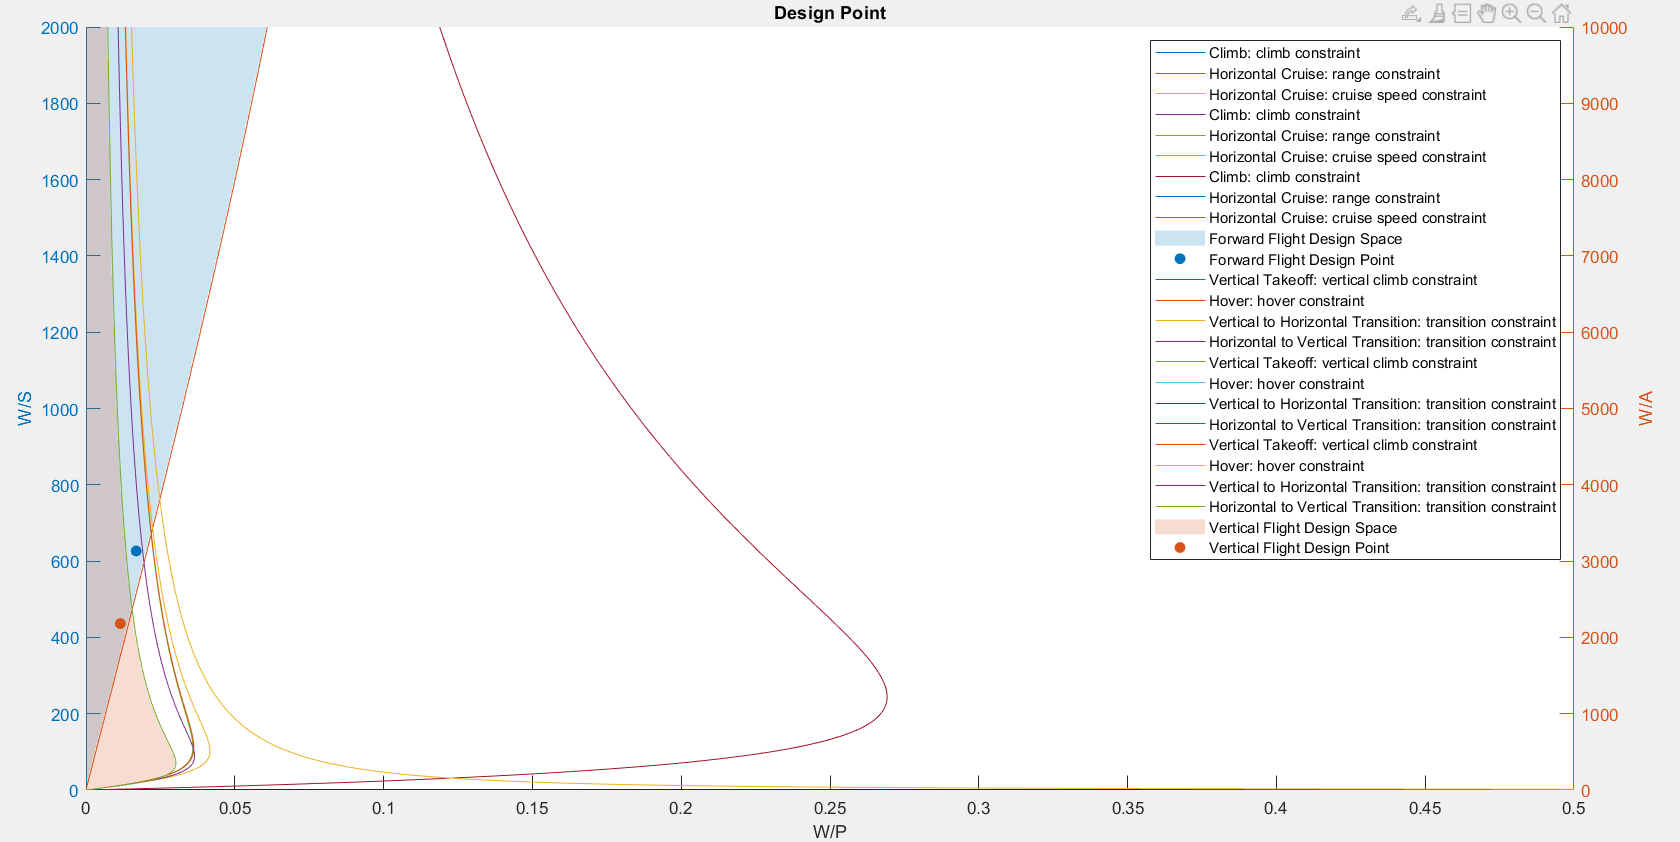
\includegraphics[width=\textwidth]{Imagens/semana6_com_brake_specific_correto_designpoint.PNG}
    \caption{Desgin Point com brake-specific fuel consumption ajustado e 700+ km de alcance- Semana 6}
    \label{designpoint_plot_semana6_correto_specifc_fuel consumption}
\end{figure}
\FloatBarrier

\section{Wing\&Tail}
\section{Engine Selection}
\section{Semana 7 - Fuselagem Design, Design Point Iteration}

\subsection{Introdução}
A semana 7 focou-se principalmente no design da fuselagem. Procurando-se ter valores concretos para as dimensões exteriores desta mesma, nomeadamente, o comprimento total e a largura. Além disto, também o interior foi concebido, focando-se na colocação dos assentos, portas, material médico, \textbf{inserir mais coisas}. Este último foi largamente baseado no AW 139.\par
O segundo objetivo da semana foi realizar iterações do design point a fim de encontrar valores que resultassem num melhor design. Para tal foi desenvolvido um programa em python que lê o json do design e aplica um algoritmo genético simples para chegarmos a um design melhor. De forma a poder automatizar a criação de novos designs, bem como a sua avaliação com o programa em python e gerar o desgin point em matlab, necessário para o algoritmo genético, foi escrito um script em poweshell. Além disto, o programa em matlab original foi modificado a fim de ser possível retirar as coordenadas do design point a fim de serem utilizadas pelo programa em python. 
\subsection{Fuselage Design - Exterior}
\subsection{Fuselage Design - Interior}
\subsection{Iteration}
A iteração foi implementada em powershell e teve a seguinte forma.:\vspace{5pt}
\FloatBarrier
\fbox{
    \begin{minipage}{\textwidth}
        \begin{itemize}
            \item Correr programa de inicialização/geração inicial de novos ficheiros json com ficheiro original como imput
            \item Fazer loop n vezes
            \begin{itemize}
                \item Correr matlab para todos os ficheiros gerados
                \item Correr programa python com algoritmo genético
            \end{itemize}
        \end{itemize}
    \end{minipage}
}
\FloatBarrier
\vspace{5pt}
O programa de inicialização tem a seguinte estrutura:
\vspace{5pt}
\FloatBarrier
\fbox{
    \begin{minipage}{\textwidth}
        \begin{itemize}
            \item Abre o ficheiro json que recebe como imput
            \item Corre n vezes
            \begin{itemize}
                \item Varia as seguintes variaveis por um valor entre $\pm0.1\% e \pm1\%$
            \begin{itemize}
                \item fuselagem - diametro
                \item asa - aspect ratio, corda média
                \item rotor - raio, rotor\_solidity
            \end{itemize}
            \item Cria ficheiro json n
            \end{itemize}
            
        \end{itemize}
    \end{minipage}
}
\FloatBarrier
\vspace{5pt}
O programa matlab corre os 10 ficheiros json criados, e gera um ficheiro de texto com as coordenadas dos design points (W/P,W/A) e (W/P,W/S) de cada json gerado.
O segundo programa escrito em python, com o algoritmo genético, tem a seguinte estrutura:
\vspace{5pt}
\FloatBarrier
\fbox{
    \begin{minipage}{\textwidth}
        \begin{itemize}
            \item Abre o ficheiro com as coordenadas dos designs points dos 10 designs gerados
            \item Calcula a figura de mérito para cada design
            \item Preserva o ficheiro com melhor figura de mérito; apaga o resto
            \item chama o programa de inicialização com ficheiro com melhor figura de mérito como input
        \end{itemize}
    \end{minipage}
}
\FloatBarrier
\vspace{5pt}
O cálculo da figura de mérito é feito através do seguinte algoritmo
\vspace{5pt}
\FloatBarrier
\fbox{
    \begin{minipage}{\textwidth}
    \begin{itemize}
        \item Se a coordenada x de (W/P, W/S) <=1300 e a coordenada y de (W/P, W/A) <=6000
        \begin{itemize}
            \item Mérito = 1/(coordenada x de (W/P, W/S))+10*(coordenada y de (W/P, W/A))
        \end{itemize}
        \item else
        \begin{itemize}
            \item Mérito = 0
        \end{itemize}
    \end{itemize}
    \end{minipage}
}
Este algoritmo tenta puxar o ponto (W/P, W/S) para a esquerda e o ponto (W/P, W/A) para cima, encontrando um equíbrio entre os dois.\par
O código de inicialização tem a seguinte forma. Aoesar de ser pouco prático de editar e poder ser feito uma implementação com loop, a falta de conhecimento sobre a linguagem python levou a que esta solução fosse criada, dado os ganhos de tempo em não aprender formas mais compactas e editáveis numa nova linguagem de programação.\par
\vspace{5pt}
\hrule
\vspace{5pt}
\FloatBarrier

    \begin{minipage}{\textwidth}
        \begin{minted}{python}
        import json
        import random
        import sys
        print(sys.argv[1])
        print()
        a_file = open(str(sys.argv[1]), "r")
        json_object = json.load(a_file)
        random.seed(a=None, version=2)
        a_file.close()
        #print(data)
        for i in range(10):
            json_object['vehicle']['components'][4]['diameter'] += random.randrange(10)/1000*json_object['vehicle']['components'][4]['diameter']*(random.randint(0,1)*2-1)
            json_object['vehicle']['components'][5]['aspect_ratio'] += random.randrange(10)/1000*json_object['vehicle']['components'][5]['aspect_ratio']*(random.randint(0,1)*2-1)
            json_object['vehicle']['components'][5]['mean_chord'] = json_object['vehicle']['components'][5]['aspect_ratio']/7
            json_object['vehicle']['components'][7]['aspect_ratio'] += random.randrange(10)/1000*json_object['vehicle']['components'][7]['aspect_ratio']*(random.randint(0,1)*2-1)
            json_object['vehicle']['components'][7]['mean_chord'] += random.randrange(10)/1000*json_object['vehicle']['components'][7]['mean_chord']*(random.randint(0,1)*2-1)
            json_object['vehicle']['components'][13]['radius'] += random.randrange(10)/1000*json_object['vehicle']['components'][13]['radius']*(random.randint(0,1)*2-1)
            json_object['vehicle']['components'][13]['rotor_solidity'] += random.randrange(10)/1000*json_object['vehicle']['components'][13]['rotor_solidity']*(random.randint(0,1)*2-1)
            #json_object['vehicle']['components'][13]['number'] += round((random.randint(0,1)-0.65))
            #json_object['vehicle']['components'][17]['number'] = json_object['vehicle']['components'][13]['number']
            with open('JSONS/data'+str(i)+'.json', 'w', encoding='utf-8') as f:
                json.dump(json_object, f, ensure_ascii=False, indent=4)
        \end{minted}
    \end{minipage}

\hrule
\vspace{20pt}
O código que calcula a figura de mérito é o seguinte:\par
\vspace{2pt}
\hrule
\vspace{5pt}
\FloatBarrier
\begin{minted}{python}
import csv
import os

meritList = []

class merit:
    val = 0
    def calc(me,a,b):
        if a <= 1300 and b <= 6000:
            me.val=1/(a)+(10*b);
        else:
            me.val=0
        
MyMerit=merit()

with open('design_points.txt', newline='') as csvfile:
    points = list(csv.reader(csvfile, delimiter=',', quotechar='|'))
    print(points[1][1])
    print()
    i=0;
    for row in points:
       MyMerit.calc(float(points[i][0]),float(points[i][3]))
       print(MyMerit.val)
       i=i+1
       meritList.append(MyMerit.val)

for k in [x for x in range(i) if x != meritList.index(max(meritList))]:
    os.remove('JSONS/data'+str(k)+'.json')

os.system("py eddit_vars.py"+' JSONS/data'+str(meritList.index(max(meritList)))+'.json')

\end{minted}

\hrule
\vspace{20pt}
O script de powershell é o seguinte:
\vspace{2pt}
\hrule
\vspace{5pt}
\FloatBarrier
\begin{minted}{powershell}
py eddit_vars.py "JSONS/prototipo3_funciona.json"
foreach($i in 1..10){
matlab -nosplash -nodesktop -r "run('ARChanges_runtrhough_underscores.m')";
Start-Sleep -Seconds 35
py secondpart_edit_vars.py
}
\end{minted}
\hrule
\vspace{20pt}
Esta implementação permitiu rapidamente passar dum design para um outro considerado melhor. É apresentado o antigo e novo design de forma a mostrar os avanços desta semana em relação ao design point.\par
\FloatBarrier
\begin{figure}[h]
        \centering
    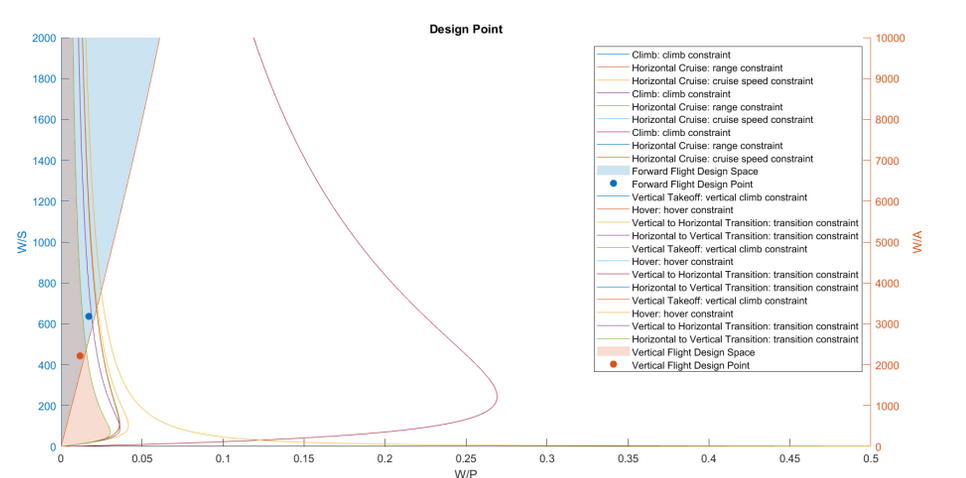
\includegraphics[width=\textwidth]{Imagens/json_1_semana7.PNG}
    \caption{Design Antigo}
    \label{json_1_semana7}
\end{figure}
\FloatBarrier
\begin{figure}[h]
     \centering
    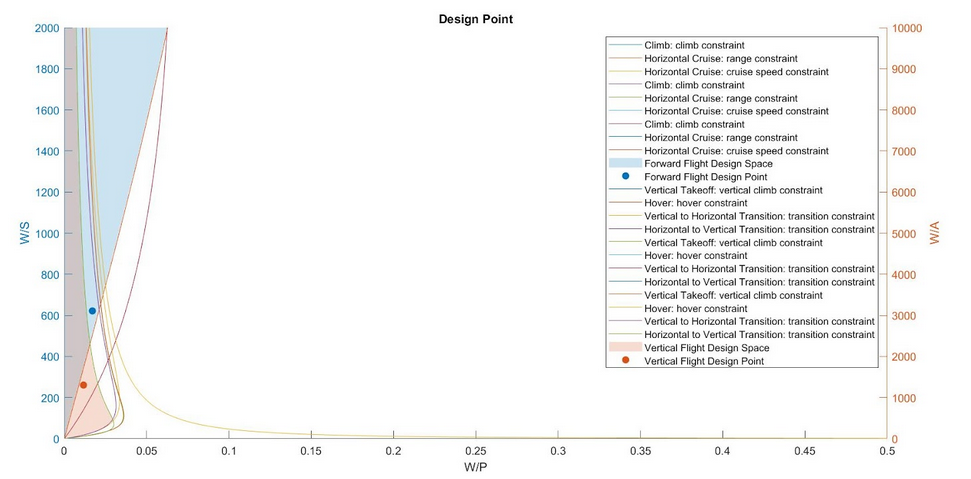
\includegraphics[width=\textwidth]{Imagens/json_2_semana7.PNG}
    \caption{Novo Design - Semana 7}
    \label{json_1_semana7}
\end{figure}
\FloatBarrier
\pagebreak
\printbibliography
\end{document}
